\documentclass[titlepage]{article}
\usepackage{illcmolthesis}
\usepackage{hyperref}
\usepackage{array}
\usepackage{amsmath}
\usepackage{cleveref}
\usepackage{biblatex} 
\usepackage{textcomp}
\usepackage[font=small,labelfont=bf]{caption}
\hypersetup{colorlinks, citecolor=black, filecolor=black, linkcolor=black, urlcolor=black}
\addbibresource{references.bib} %Import the bibliography file

\begin{document}


\title{Mathematically Modeling the Interactions Between Phages,  Bacteria, and the Environment}
\author{Victor J. Piaskowski}
\birthdate{August 2, 2001}
\birthplace{Royal Oak, MI, USA}
\defensedate{June 27, 2025}
\supervisor{Dr. Matti Gralka}
\committeemember{Dr. Matti Gralka}
\committeemember{Dr. Jaap Kaandorp}
\committeemember{Dr. Yuval Mulla}
\pagenumbering{roman}
\maketitle
\begin{abstract}
    Abstract text here
\end{abstract}
\newpage

Abbreviations of terms

\begin{table}[ht!]
    \begin{tabular}{|l|l|}
        \hline
        Abbreviations & Full Word                         \\ \hline
        ODE/s         & Ordinary Differential Equation/s \\ \hline
        DDE/s         & Delay Differential Equation/s \\ \hline
        PDE/s         & Partial Differential Equation/s \\ \hline
        BVP  & Boundary Value Problem \\ \hline
        ABM/s  & Agent Based Modelling/Models \\ \hline
        -  & - \\ \hline
    \end{tabular}
\end{table}

\newpage

\tableofcontents
\newpage 
\pagenumbering{arabic}
\section{Introduction}
\label{sec:Introduction}
\chapter{Introduction}
\label{Introduction}

Phages are small viruses on the order of 27-190nm that infect and lyse (kill) specific bacteria, acting as nature's natural anti-microbial defense. 
Researchers are attempting to determine how phages can be used in various medical and industrial applications to control bacterial growth. 
However, researchers need to know how the interactions between phages and bacteria work in order to implement a robust method to control bacterial growth. 

\section{Thesis Overview}
This thesis covers multiple topics to ultimately answer how phages and bacteria interactions can be mathematically modelled. 
First, there is a (biological) introduction to phages and bacteria. 
This introduction covers how phages work and infect bacteria, how bacteria defend against phages, how phages defeat bacterial defenses, and how phages defend against other phages. 
There is also an introduction to different modelling techniques such as spatial vs non-spatial models and ODEs vs DDEs. 
This thesis briefly covers software that models phages, resources, bacteria, and their limitations. 

This thesis presents software I developed to support the research, demonstrating its capabilities using a representative model of phage-bacteria-resource interactions. 
The section also provides an overview of its usage, including example outputs from demonstration runs.
Finally, the results generated by the software will be thoroughly analyzed and discussed.

\section{Biological Background}
Phages are small viruses on the order of 27-190nm (the average size of marine phages are 54nm) that infect and lyse (kill) specific bacteria.
Phages are so small, that it takes 55 million phages to cover the period at the end of this sentence \cite{breitbartPhagePuppetMasters2018}. 
The phage cycle process starts with a phage coming into contact with a bacterium.
Once it has identified an injection site, the phage can inject a strain of DNA into the bacteria.
The DNA strand has two options: it can either merge into the bacterial DNA, allowing the phage's DNA strand to replicate alongside the bacteria as they reproduce.
This process defines the Lysogenic cycle.
After a set amount of time, the DNA of the phage can unmerge and hijack the DNA replicating mechanism, creating multiple copies of itself, using the transcription, translation, and replication process to create multiple copies of itself.
The phages begin to self-assemble inside the bacteria until the bacteria is full of phages and explodes, the lysis stage, releasing the phages into the environment, ready to repeat the process again. 

This process can be visualized in \Cref{fig:phage_life_cycle}.
\begin{figure}
    \centering
    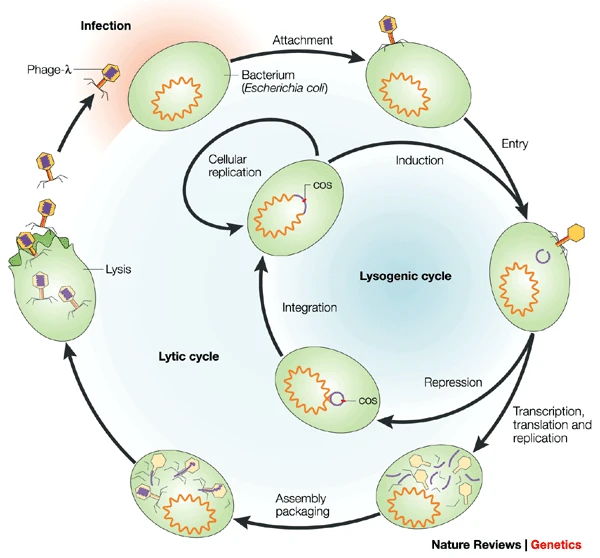
\includegraphics[width=0.5\linewidth]{Figures/phage_life_cycle.png}
    \caption{Life cycle of a phage, inside and outside a bacteria cell. Significant steps in the life cycle of a phage include the infection stage, integration, replication, and lysing process. Figure sourced from \citet{campbellFutureBacteriophageBiology2003}. }
    \label{fig:phage_life_cycle}
\end{figure}

\section{The Environment}
In an ecosystem like the ocean, the gut, or in soil, there are thousands of different microbes all interacting with one another or the surrounding environment.
The interactions are complex, with many factors affecting the growth of bacteria, phages, plants, animals, and more. 

The interactions between entities in the environment are often synergistic. 
When an animal dies, bacteria start to digest and decompose the animal into simpler chemicals like carbon and nitrogen that plants can use to grow, which is then eaten by other animals. 
External factors, such as flooding, droughts, chemical spills, or introduction of new entities have a massive impact on the ecosystem. 
These events can add or remove resources from the system, change environmental parameters such as the surrounding temperature, introduce competition, or create an imbalance in the population by killing entities. 
These effects have a larger effect on the ecosystem and food chain as a whole as bacteria are one of the fundamental foundations for resource recycling. 

\subsection{Phage's Role in the Environment}
Phages play a large role in the ecosystem. 
As bacteria die, for example through lysis, they release resources into the environment for other bacteria and plants to use. 
This turns over resources like nitrogen and carbon for other sources to use. 
Phages also help mediate horizontal gene transfer, disperse pathogenic diseases, and spread antibiotic resistance \cite{al-shayebCladesHugePhages2020}. 
Phages directly alter bacteria population diversity and population fitness by introducing new ways for bacteria to mutate \cite{brownEcologicalFunctionalRoles2022}. 
There are about $10^6$ bacteria cells/ml and $10^7$ phages/ml of marine water. 
About 5\% of any bacteria are currently infected and about 15\% of daily bacterial death can be attributed to phages \cite{chibani-chennoufiPhageHostInteractionEcological2004}. 


Phage populations depend on growth by infection and death by degrading. 
UV is a large factor of killing marine phages, causing up to a 5\% reduction in phage infectivity per hour \cite{chibani-chennoufiPhageHostInteractionEcological2004}. 

\subsubsection{Phages and Controlling Bacterial Blooms}
Phages could potentially be used to control \textit{Cyanobacteria} (blue-green algae) blooms in the environment \cite{colomaFrequencyVirusresistantHosts2019}. 
\textit{Cyanobacteria} cause damage to aquatic life by consuming resources and oxygen, starving aquatic life and negatively affect human health. 
There is hope that phages can be used to biologically control water quality in waste water treatment plants and in the environment without the use of harsh chemical processes what would otherwise pose environmental and health hazards \cite{krysiak-baltynSimulationPhageDynamics2017, tuckerIdentificationCyanophageMaLBP2005}. 
More information about controlling \textit{Cyanobacteria} can be read in \nameref{sec:AppendixB:environmental_protection}. 

\section{Phage Cocktails and Human Health}
There is particular interest in phage applications in human and animal health, called phage cocktail therapy, due to phage cocktails not exhibiting side effects.
Phage cocktails are a medicine that sick patients with bacterial diseases, such as \textit{Escherichia coli} can use. 
A patient can swallow a pill filled with a range of different phages that target \textit{E. coli}.
The phages will target the specific \textit{E. coli} bacteria, but it will not affect the other bacteria found in the gut of the human body and will not have any side effects on the body. 
There are about 100 trillion microbes across 5,000 different types of bacteria strains in the human gut. 
Antibiotics disrupt the intricate ecosystem of the gut microbiome, acting as a scorched-earth mechanism. 
Phages on the other hand specifically target a specific bacterial strain, acting as a sniper, with minimal to no effects to other bacterial strains, while antibiotics act as a bomb. 
A challenge that antibiotics face is that antibiotics create antibiotic resistant bacteria, making the antibiotic less effective in the future \cite{odonkorBacteriaResistanceAntibiotics2011, volkovaEffectsEarlylifePenicillin2021}. 
There is however hope that phage resistant bacteria become more susceptible to antibiotics due to changes in the cell structure \cite{laurePhageResistancemediatedTradeoffs2022, zhaoPhagedrivenCoevolutionReveals2024}. 
\nameref{sec:AppendixB:phage_therapy_and_antibiotics} in \nameref{AppendixB} goes more in depth on how phages can be used in a healthcare setting. 

\section{Industrial Usage}
Phages have many uses in an industrial setting. 
Similarly, phage therapies can be used as a preventative method, by preventing the spread of common bacteria in livestock by dosing the animal feed with the phage pills. 
Farmers often raise livestock in tight spaces with a lack of sanitation facilities, increasing the risk of a disease spreading. 
 
Phages can be used to control the growth of bacteria like \textit{Salmonella} while producing food in a factory \cite{sofferBacteriophagesSafelyReduce2016, kowalskaFreshVegetablesFruit2023}. 
\nameref{sec:AppendixB:controlling_foodborne_bacteria} in \nameref{AppendixB} goes into more detail about using phages to control foodborne bacteria. 

\section{Modelling Phages in a Complex Community}
Not much is known about phages in large and complex communities between other phages, bacteria, resources, and the environment. 
There have been previous attempts to model the complex dynamics of the populations between phages, bacteria, and resources, with the environment using Ordinary Differential Equations (ODE) and Delay Differential Equations (DDE).
Not every interaction in the complex community can be identified, and if an interaction has been identified, the associated parameter values are unknown and need to be experimentally derived. 
Collecting interaction parameter values is an expensive and laborious task, as the data has to experimentally collected. 

There are two main ways to model phage-bacteria dynamics: spatially and non-spatially.
In a spatial model phages and bacteria can move through space and interact with their neighbors. 
Partial differential equations (PDE) and cellular agent-based models (ABM) have been used to model spatial interactions.
Spatial models require special considerations, such as proximity to other entities.
This creates areas of interaction and interest where entities are located, and areas of no interactions where there are no interactions.
Spatial models lead to more computationally complex models, but can result in more interesting and biologically realistic results. 

Whereas in non-spatial models such as ODEs and DDEs, the bacteria and phages are assumed to be in a well-mixed solution and no distinctions are made in regard to neighbors or distances to other entities. 
Interactions are simplified to a probabilistic approach, where a percentage $p$ of entities interact with one another at time step $t$.
Non non-spatial models are easier to develop, understand, and are more effective in modeling large populations, at the cost of losing spatial information. 

For this thesis, the focus will be modelling resource, phage, and bacteria interactions using an ODE model. 
A phage-bacteria-resource system is described as an $p\times b \times r$ system, meaning $p$ phages, $b$ bacteria, 
Current modelling methods have mainly stayed with $1\times 1 \times 1$ models, meaning 1 phage, 1 bacteria, and 1 resource. 
This thesis aims to develop a simulation framework that can model any $p\times b \times r$ ODE system, where each entity can contain states (called hidden entities) that they can move to and from. 
\newline 

\section{Software Overview}
The project is divided into three logical parts, with an optional fourth part.
The first section is to create the network interaction. 
Here the user of the software can define the number of resources, phages, and bacteria, who interacts with who, and the strength and type of interactions. See \nameref{sec:network_creation_tool} for further information. 
In \nameref{sec:simulation_framework}, the user uploads the network model and parameters and as output receives the time data and population data as an array. 
\nameref{sec:visualization_framework} allows the user to interact with \nameref{sec:network_creation_tool} and \nameref{sec:simulation_framework} with a dashboard. 
The user can graphically edit the attribute values of the edges and nodes of the network, and the user can run more advanced visualizations, for example by changing a parameter value and seeing how that affects the population count. 
There are a few plots included out of the box that the user can test. 
The plots offered in part 3 offer interactivity like hiding and showing lines and dots, zooming in and out, and hovering over the lines and dots to show more details of the data. 

Finally, the user can optionally run multiple simulations and download the data to their disk to create their own custom visualizations using \nameref{sec:custom_visualizations_and_framework}. 
The visualizations created in \nameref{sec:visualization_framework} can theoretically be recreated in \nameref{sec:custom_visualizations_and_framework}. 
The user can choose the same parameter values used for a specific plot in \nameref{sec:visualization_framework}, run the simulation (under the \nameref{sec:ultimate_analysis} section), download the data, and reimplement the graphs. 

The user can use the tool themselves by importing the Python classes in their own code and initializing the classes and passing the appropriate data. 
\newpage

\section{Literary Review}
\label{sec:Literature}
\subsection{Methods of Modelling Phages and Bacteria}
There are numerous ways to model the interactions between phages and bacteria. Models can be built at a molecular level, where the model simulates the mechanical and chemical behavior of a phage as it interacts with the surface of a bacterium using computational chemistry methods. On the other end of the spectrum, a different type of model can be built where populations of phages, bacteria and bacteria can be modeled using Ordinary Differential Equations (ODEs) or Delay Differential Equations (DDEs). DDEs are similar to ODEs, except where when ODEs are calculating the values of the equations at time $t$ using time $t-1$, DDEs can, but don't have to, use the value of the equation at time $t-\tau$, where $1 \leq \tau \leq t$. \newline 

Each type of system has its pros and cons. With the molecular level model, the model is more complex and needs significantly more startup time, simulation time, and is in general much more complex. However, more information can be gained from the simulations and can guide research in creating phages for a certain type of bacteria. The ODE method is simpler and easier to set up, however it can only capture large population dynamics. Certain assumptions have to be made, for example $\omega$ percent of the bacteria population is washed out. The model can be made more complicated, by modelling each stage of a lysis, or when calculating the washout rate of bacteria, use a normally distributed variable $\textbf{N}(\mu=\omega, \sigma=1)$ to capture slight variations in a parameter at each step to controllably randomize parameter values to capture noise in measuring data. Ensuring the use of a seed value will ensure that each run of the model results in the same output. 

\subsubsection{Generalized Lotka-Voltera Model}
The Lotka-Voltera model, a first-order non-linear differential model is a model that captures the dynamics between predators and prey, with phages being the predator and bacteria being the prey. Any population can be modelled as such
\[ 
    \frac{d{B}_i}{dt} = {B}_i \left(\left(r_i + \sum_{j}^{N} \alpha_{ij}{B}_j \right) - m_i\right)
\]
where ... there is a typo. 

\subsubsection{Generalized Consumer-Resource Model}
The generalized Consumer-Resource Model models the growth of a population and resource dynamics between a population of bacteria ${B}_i$ and a resource ${R}_i$. 
\begin{align}
    \frac{d{B}_i}{dt} &= r_i{B}_i \left(\sum_{\alpha} \Delta w_{i \alpha}C_{i \alpha}R_{\alpha}\right) - m_i {B}_i \\
    \frac{R_{\beta}}{dt} &= -\sum_i C_{i\beta}R_{\beta}{B_i} + \sum_{\alpha, i}D_{\beta\alpha}^{i}C_{i\alpha}R_{\beta}{B}_i \\
    \Delta w_{i\alpha} &= \sum_{\beta}D_{\beta \alpha}^{i}w_{\beta}
\end{align}

\subsubsection{Trait-Based Model}
The Trait-Based Model is a model that takes into account external factors such as the temperature or pH of the system, and can be modeled as following:  
\begin{align}
    \frac{dB_i}{dt} &= \left(r_i - m_i\right) B_i \\
    r_i &= \frac{r_{i\alpha}^{max}R_\alpha}{R_\alpha + K_{i\alpha}}e^{S_i\left(T-T_{ref}\right)}
\end{align}
where $S_i$ is the sensitivity to $B_i$ to factor $T$, and with tradeoff if $r_i^{max} > \text{ mean } r^{max} \text{ then } S_i > \text{ mean } S$. 

\subsubsection{Agent-Based Models}
Agent-based Models (ABM) model the system through space and time. An $x \times y \times z$ grid (often $z$ is left out for a 2D system) is created and split into smaller subcells containing resources and microbes. Each cell acts as its own tiny environment, where resources and microbes interact within the environment, but not with the neighboring cells. Resources are diffused through the system using a PDE solver for a Boundary Value Problem (BVP). Agents are allowed to move into neighboring grids with a probability $p$, where $p$ can depend on any number of parameters such as nutrient density, microbe density, or stochastic chance. \newline 
ABMs are useful when simulating many individual elements interacting in a system. Chaotic or emergent behaviour can arise from these interactions. Chaotic behavior refers to the irregular and unpredictable evolution of a system's behavior due to nonlinear equations, exhibiting sensitive dependence on initial conditions \cite{encyclopedia_of_physical_science_and_technology}. \newline 
Emergent behavior is something that is a nonobvious side effect of bringing together a new combination of capabilities—whether related to goods or services. Emergent behaviors can be either beneficial, benign, or potentially harmful, but in all cases they are very difficult to foresee until they manifest themselves. Agents can have simple rules, but when interacting with other agents, behavior that hasn't been programmed can arise. Emergent behaviors are also sometimes considered to be systems that are more complex than the sum of their parts \cite{macaulayThreatsImpactsIoT2017}. 



\begin{align} 
    \frac{\delta R_\alpha(r, t)}{\delta t} = \nabla \left[D \left( R_\alpha, r\right) \nabla R_\alpha \left( r, t \right) \right], r = \left(x, y\right)
\end{align}. 
The cellular agents rules are as follows. 
\begin{align} 
    \frac{di}{dt} = r_i \left( \sum_\alpha \Delta w_{i\alpha}C_{i\alpha}R_\alpha\right)
\end{align}, where if $i>$ threshold, $\frac{i}{2}$ expands into the neighboring grid cell with a probability $p$. 
The resource consumption and conversion into new sub-resource types are described as follows. 
\begin{align}    
    \frac{dR_\alpha}{dt} &= -\sum_i C_{i\alpha}R_\alpha I \\
    \frac{dR_\beta}{dt} &= \sum_i C_{i\beta}R_\beta I + \sum_{\alpha, i}D_{\beta \alpha}^{i} C_{i \alpha} R_\alpha i
\end{align}






\subsection{Biology of Phages}
\subsubsection{Current Applications: Food Control}

When there are small number of known bacterial strains, a targeted concoction of phages can be used to control the bacterial population growth on the food. Phages offer properties of microbial control that other methods do not. Phages do not modify the food quality and do not leave behind harmful chemical residues. Phages are hyperspecific to the bacteria that they can kill, and they don't affect other beneficial bacteria. For example, \textit{Streptococcus thermophilus} is one of three different bacteria strains used to create emmental cheese. However, Emmental cheese does not use pasteurized milk, increasing the risk of \textit{E. coli}. Emmental cheese producers can add phages that target \textit{E. coli} to the milk during the production stage while not affecting the bacteria used to produce the cheese. \newline 


Phage cocktails like SalmoFresh\textsuperscript{TM} have been proven to safely reduce \textit{Salmonella} contamination in pet food and raw pet food ingredients \cite{sofferBacteriophagesSafelyReduce2016}, as well as in romaine lettuce and bean sprouts \cite{zhangSalmoFreshEffectivenessControlling2019}. Pet food contains meat and vegetables, where vegetables grown in or on the ground are at risk of \textit{Salmonella} due to contact with soil, manure, compost, and other agricultural runoff from neighboring farms \cite{kowalskaFreshVegetablesFruit2023}. \Cref{fig:SalmoFresh_pet_food} \cite{sofferBacteriophagesSafelyReduce2016} and \Cref{fig:SalmoFresh_lettuce} \cite{zhangSalmoFreshEffectivenessControlling2019} show how applications of phages have reduced the count of \textit{Salmonella} in ingredients used in pet food as well as romaine lettuce and bean sprouts. As such, phages can be shown to control the spread of \textit{Salmonella} in food sources. 

\begin{figure}
    \centering
    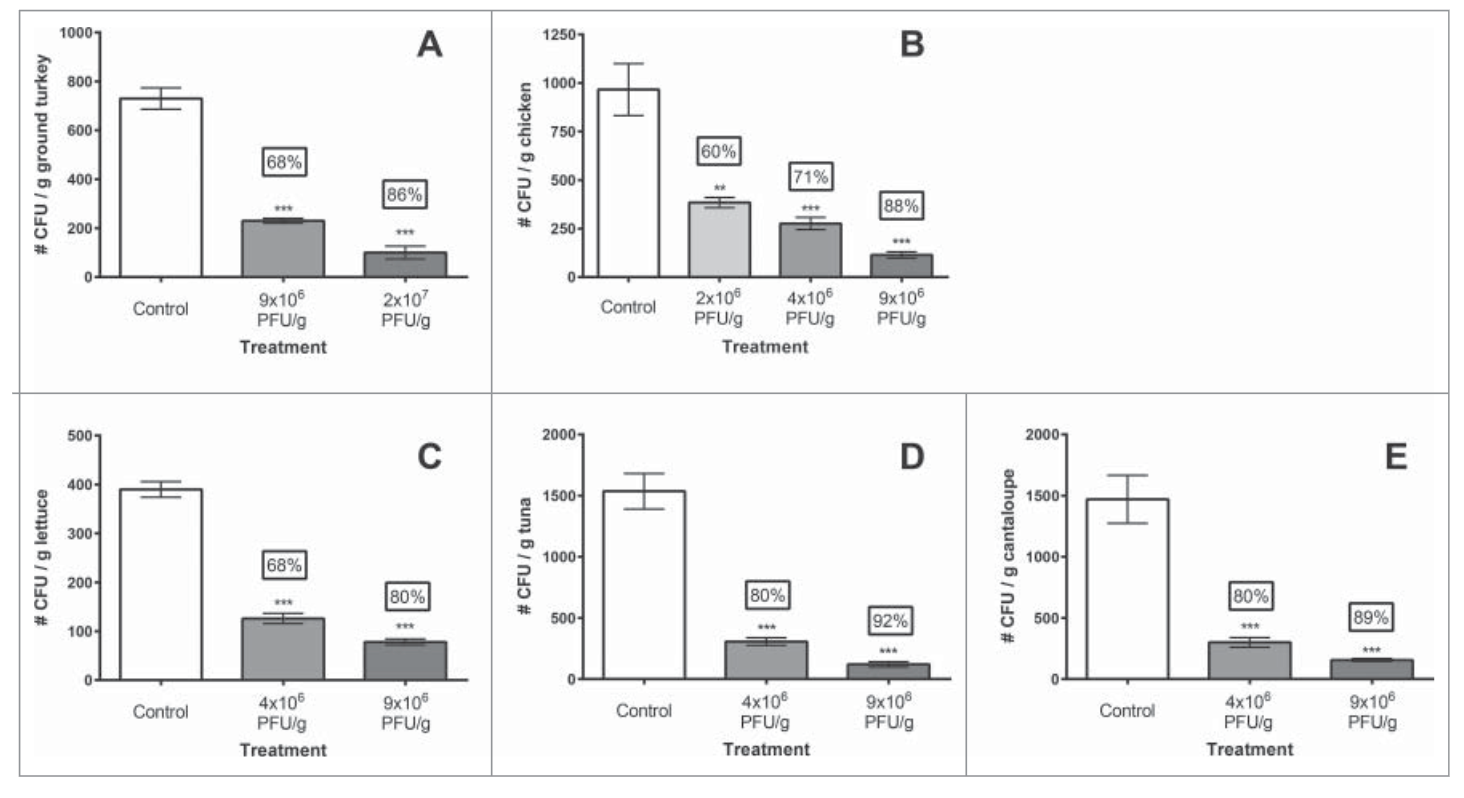
\includegraphics[width=0.5\linewidth]{Figures/SalmoFresh_in_pet_food.png}
    \caption{SalmoLyse\textsuperscript{\textregistered} reduces Salmonella contamination on various food surfaces: Mean and standard error bars shown. Statistical analyses were carried out for each food group independently. Asterisks denote significant reduction from corresponding controls based on one-way ANOVA with Tukey’s post-hoc tests for multiple corrections: ** denotes $p < 0.01$, while *** denotes $p < 0.001$ compared to the corresponding controls. There was significant reduction in Salmonella on all food surfaces with the addition of SalmoLyse\textsuperscript{\textregistered} compared to the controls; the mean percent reductions from the control are noted in the boxes above treatment bars. CFU/g D colony forming units per gram. Each letter denotes a food group that was tested with SalmoLyse\textsuperscript{\textregistered} and compared to a control: A= chicken; B= lettuce; C= tuna; D= cantaloupe; E= ground turkey. \cite{sofferBacteriophagesSafelyReduce2016}}
    \label{fig:SalmoFresh_pet_food}
\end{figure}

\begin{figure}
    \centering
    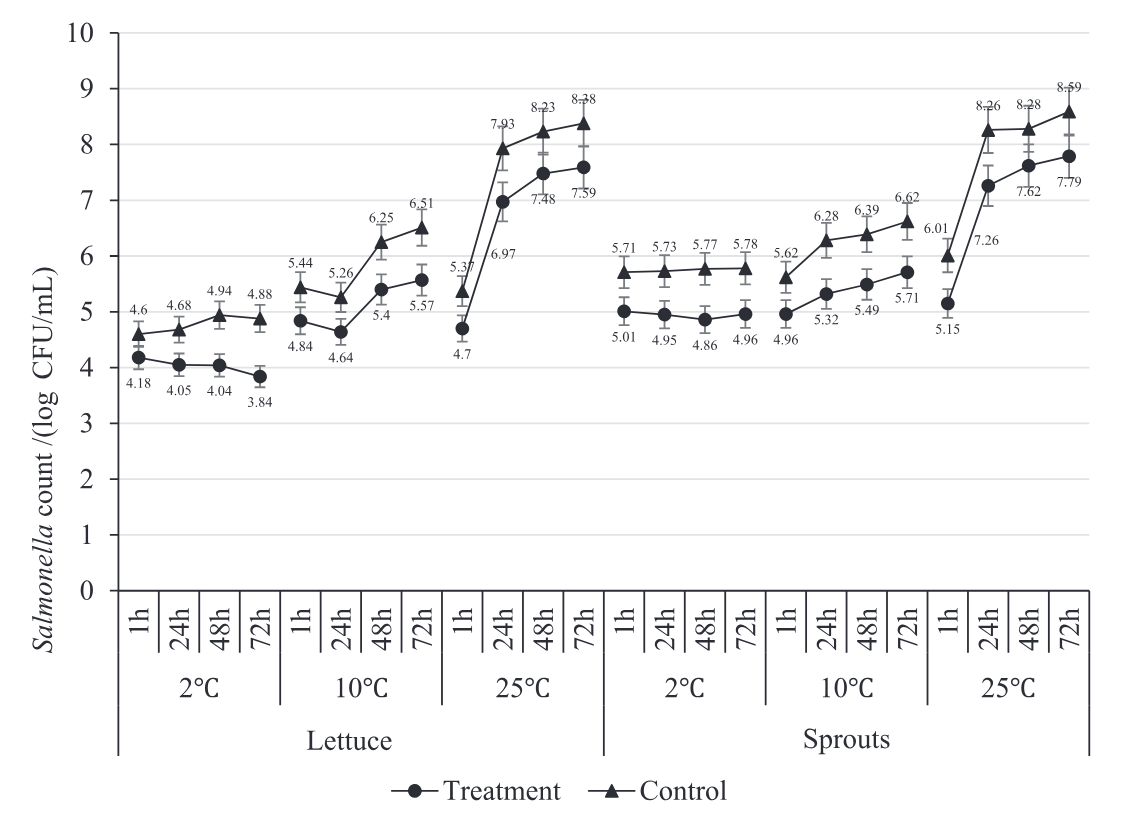
\includegraphics[width=0.5\linewidth]{Figures/SalmoFresh_effectiveness_lettuce_sprouts.png}
    \caption{\textit{Salmonella} count in a mixture of 5 \textit{Salmonella} strains spot-inoculated (CFU/g) onto a) lettuce and b) sprouts after spraying with a mixture of bacteriophage (SalmoFresh\textsuperscript{TM}) relative to positive controls at 2, 10 and 25C and stored for 1, 24, 48 and 72 h. \cite{zhangSalmoFreshEffectivenessControlling2019}}
    \label{fig:SalmoFresh_lettuce}
\end{figure}


\subsubsection{Current Applications: Bacterial Infection Control}


\subsubsection{Current Applications: Environmental Control}
There is interest in using phages to control cyanobacteria blooms. Phages can offer better and safer options than chemical options. Chemical options are indiscriminate, killing cyanobacteria, while also killing other beneficial bacteria and aquatic life. Although not used to control bacteria blooms, some chemicals like PFAS, also called "Forever Chemicals", can last a long time in the environment and don't degrade and keep on negatively affecting the environment. Due to the specificity of phages, only the cyanobacteria will be targeted, and will not affect the surrounding areas. Tucker and Pollard found that an isolated phage cocktail collected from Lake Baroon in Australia could decrease the abundance of \textit{M. aeruginosa} by 95\% within 6 days in a lab setting, before recovering within 3 weeks time \cite{tuckerIdentificationCyanophageMaLBP2005}. \newline 
There is evidence that phage-resistant bacteria can influence the population dynamics of other bacteria. It has been shown that the plankton level has been experimentally affected by the frequency of the phage-resistant \textit{Nodularia} marine bacteria. Populations with high phage resistance ($>50\%$) dominate the plankton communities despite a high phage count and eventually outcompete other bacteria due to their slower loss in population count. Contrastingly, populations of bacteria with low phage resistance (between 0\% and 5\%) were lysed to extinction, releasing nutrients like nitrogen. This allows for other bacterial strains to absorb the nutrients and dominate the bacterial community. Phages and the lysis of bacterial strains can have a dramatic effect on community dynamics and composition of other agents like phages, bacteria, and resources \cite{colomaFrequencyVirusresistantHosts2019}. Phages have the potential to be used as a highly specific strategy for the control of cyanobacterial blooms, with minimal effects to the environment, and offer control bacterial blooms, with limited impact to the environment. Usage should be relatively safe, novel, efficient, and sensitive. \newline 

However, there are issues with using phages to control bacterial blooms. Bacterial blooms can cover vast areas, or be in areas that would be hard to reach like marshlands, applying phages to combat the bloom might be infeasible. If the method of choice was to spray a solution of water containing phages, the solution needs to be shipped to the site and loaded onto special boats to  spray the solution into the water, or the trucks need to drive along the shore and spray the solution into the water. The phage density in the solution will have to be relatively high to quickly combat the bloom. These problems provide major logistical problems with creating the phages in a lab or factory, transporting the phages, and finally the administration of the phages to the waterways. Phages can only diffuse through the water, and can't actively swim, so they are dependent on the rate of diffusion and water currents. This will be difficult in marshlands, where the bacteria can "hide" in the grass and crevices created by aquatic life. If the bloom is in a high current area, like in a river or a bay, the water can wash the phages away. On top of that, The infection mechanism of phages is not exactly known, and research into artificial engineering of phages is not in-depth, making it harder to do research in this area \cite{grassoReviewCyanophageHost2022, DissolvedMicrocystinRelease}. 
\newpage

\section{Methods}
\label{sec:Methods}
\chapter{Methods}
\label{Methods}
\section{Project Overview}
To help complete this Master thesis, I created various tools that would help create the final model outputs.
The project is divided into four parts. 
The first part is the tool that a user can use to design and create the network of agent interactions. 
The second part is the simulation framework that handles the data and runs the ODE solving method. 
The third part is a dashboard that runs in the browser. The dashboard allows for a user to interact with the model, for example by changing parameter and environment values, and run some basic simulations and receive different plots as output. 
The final part allows the user to download the simulation data to create their own custom graphs and analyses. 

A flowchart showing the user-system interactions can be seen in \nameref{AppendixC}. 

\section{The Golden Model}
\label{sec:golden_model}
In this report, the default model, called the “Golden model“ \cite{gengUsingBacterialPopulation2024} that will be used for all simulations is as follows:

% \begin{equ}[!ht]
%     \begin{equation}
%         \frac{dR}{dt} &= -e \cdot g(R, v, K)\cdot (U + \sum_{i=1}^{M} I_M) \mathcolor{red}{+ w^i -w^o \cdot R}\\
%         \frac{dU}{dt} &= g(R, v, K)\cdot U - r\cdot U \cdot P \mathcolor{red}{-w^o \cdot U}\\
%         \frac{dI_1}{dt} &= r\cdot U \cdot P - \frac{M}{\tau}\cdot I_1 \mathcolor{red}{-w^o \cdot I_1}\\
%         \frac{dI_k}{dt} &= \frac{M}{\tau}(I_{k-1}-I_k) \mathcolor{red}{-w^o \cdot I_k}\text{ for } k=2, \dots, M \\
%         \frac{dP}{dt} &= \beta \cdot\frac{M}{\tau} \cdot I_M - r\cdot(U + \sum_{i=1}^{M} I_M)\cdot P \mathcolor{red}{-w^o \cdot P} \\
%         g(R, v, K) &= \frac{v\cdot R}{R + K}
%     \end{equation}
%     \caption{Caption of the equation}
% \end{equ} 

\begin{eqfloat}
    \begin{align}
        \frac{dR}{dt} &= -e \cdot g(R, v, K)\cdot (U + \sum_{i=1}^{M} I_M) \mathcolor{red}{+ w^i -w^o \cdot R}\\
        \frac{dU}{dt} &= g(R, v, K)\cdot U - r\cdot U \cdot P \mathcolor{red}{-w^o \cdot U}\\
        \frac{dI_1}{dt} &= r\cdot U \cdot P - \frac{M}{\tau}\cdot I_1 \mathcolor{red}{-w^o \cdot I_1}\\
        \frac{dI_k}{dt} &= \frac{M}{\tau}(I_{k-1}-I_k) \mathcolor{red}{-w^o \cdot I_k}\text{ for } k=2, \dots, M \\
        \frac{dP}{dt} &= \beta \cdot\frac{M}{\tau} \cdot I_M - r\cdot(U + \sum_{i=1}^{M} I_M)\cdot P \mathcolor{red}{-w^o \cdot P} \\
        g(R, v, K) &= \frac{v\cdot R}{R + K}
        \label{eq:golden_model}
    \end{align}
    \caption{
        The golden model taken from \citet{gengUsingBacterialPopulation2024}. 
        The text in red has been added to model adding (the wash-in) fresh resources ($\omega^i$) 
        and the removal (wash-out) of agents $\omega^o$. By default these values are 0.
        A summary of the parameter meanings can be found at \Cref{tab:parameter_table_simple_golden_model}. 
    }
\end{eqfloat}

where $R$ is resources, $U$ is uninfected bacteria, $I_{1, \dots, M}$ is the infected stage of the bacteria, and $P$ is the phage population. 

The model describes three biological processes, cell consumption of resources and growing, phage/cell encounters and infection, and cell lysis. 
The cell growth process is described by $g(R, v, K)$, the instantaneous growth rate dependent on the Monod equation, where $v$ is the maximal growth rate and $K$ is the Monod constant. 
The consumption rate of a resource by a bacteria is $e$. 

Once infected by a phage, the bacteria goes from $U$ to $I_1$. 
The bacteria goes through $M$ stages of infection $I_1, \dots, I_M$ before lysing, where the bacteria goes from state $I_k$ to state $I_{k+1}$ with equal transition rate $\frac{M}{\tau}$. The probability of a successful infection of a cell is $r$. 
After a bacteria lyses after stage $I_M$, $\beta$ phages are released, the burst size of the phage. 

However this model is specifically designed for a $1\times 1 \times 1$ model. 
In order to adapt this model to fit an $p \times b \times r$ model, the model needs to be slightly adapted. 
There are other changes that can be made, to the model, for example by adding a washin rate $\omega^{i}$, where resources are constantly being introduced, and a washout rate $\omega^{o}$ where all agents are washed out at a constant rate. 

\subsection{The Adapted Golden Model}
\label{sec:adapted_golden_model}
The adapted model accounts for the interactions of multiple agents. 
\begin{eqfloat}
    \begin{align}
        \frac{dR_r}{dt} &= -\sum_{b \in B} e_{b, r} \cdot g(R_r, v_{b, r}, K_{b, r})\cdot (U_b + \sum_{i=1}^{M} I_{i_b}) + w^i_r - w^o \cdot R_r\\
        \frac{dU_b}{dt} &= U_b \cdot \sum_{r \in R} g(R_r, v_{b, r}, K_{b, r}) - U_b \cdot \sum_{p \in P} r_{p, b} \cdot P_p - w^o \cdot U_b\\
        \frac{dI_{b_1}}{dt} &= U_b \cdot \sum_{p \in P}r_{p, b} \cdot P_p - \frac{M}{\tau_b}\cdot I_{b_1} - w^o \cdot I_{b_1}\\
        \frac{dI_{b_k}}{dt} &= \frac{M}{\tau_b}(I_{b_{k-1}}-I_{b_k}) - w^o \cdot I_{b_k}\text{ for } k=2, \dots, M \\
        \frac{dP_p}{dt} &= \sum_{b\in B}\beta_{p, b}\cdot\frac{M}{\tau_b} \cdot I_{b_M} - r_{p, b}\cdot(U_b + \sum_{i=1}^{M} I_{b_i})\cdot P_p - w^o \cdot P_p\\
        g(R_r, v_{b, r}, K_{b, r}) &= \frac{v_{b, r} \cdot R_r}{R_r + K_{b, r}}
        \label{eq:adapted_golden_model}
    \end{align}. 
    \caption{
        Probability of phage infection $r_{p, b}$ is not to be confused with $R_r$, short for Resource $r$. 
        The interactions are a sum of all interactions due to all interactions taking place at the same time. 
    }
\end{eqfloat}

\subsection{Network Creation Tool}
\label{sec:network_creation_tool}
The network creation tool is the first step that a user needs to use, and it revolves around using a GUI tool built to create and edit the graph representation of the agent interaction.
Numerous interactions occur between agents in a microbial environment.
However, not every agent can and will interact with one another.
Based on which agents interact with one another, a network topography representing the agent interactions and dynamics can be created. 

Every node represents a unique agent, and each agent has their own intrinsic properties. 
The user can intuitively define agents, their interactions, environmental and model settings using the GUI tool. 
This tool allows users to quickly and intuitively define agents and their attributes, agent interactions and their attributes, environmental data, and model settings.
An edge links two agents together if there is an arbitrary interaction occurring between the agents, with the properties exhibited in the interaction dependent on the interacting agents. 
Self interactions are allowed in the network. 
There is an environment node that is used to store global environmental data, such as the temperature and pH of the system.
The settings node holds information such as simulation length, max time step, and the type of ODE solver to use.
The tool provides functionalities for adding, editing, and visualizing nodes and edges, as well as importing and exporting the network structure.  

Once the user is happy with the graph shape, they can export the network representation for use in \nameref{sec:simulation_framework}, \nameref{sec:visualization_framework}, and \nameref{sec:custom_visualizations_and_framework}. 
The most important part is that the user defines the shape and the attributes of the network, as that can't be edited in part 2 onwards. 
It is possible go back to the network creation tool and upload the graph to the tool to be able to edit the network representation. \newline
The user can edit the values of the attributes in \nameref{sec:visualization_framework}, so the parameter values do not have to be perfect. 
As such, the user does not need to keep on using the GUI tool to edit parameter values. 

\Cref{fig:ss:initial_startup_GUI_tool} shows the layout of the GUI tool. \Cref{fig:ss:example_network} shows an example network that can be created.
There are numerous buttons that can be used to edit the graph, for example adding or removing nodes and edges. 
By default, an environment node holding parameters such as pH and temperature is added.
A settings node is added as well, holding settings data to be used for the solver, like the type of solver or simulation length.
Manually adding nodes and edges can get tedious and repetitive for large graphs, so the user can add multiple nodes and edges at the same time.
Nothing can interact with the environment and setting node, as they are used to hold data about the environment and network solver.
The user can alter the default attribute name and value by importing the GUI tool class and overriding the method implementation implementing the default names and values. 
The user can self-decide which parameter values to give, and if and how the parameter values are randomized. 

\begin{figure}
    \centering
    \begin{subfigure}{0.49\linewidth}
        \centering
        \captionsetup{width=1\linewidth}
        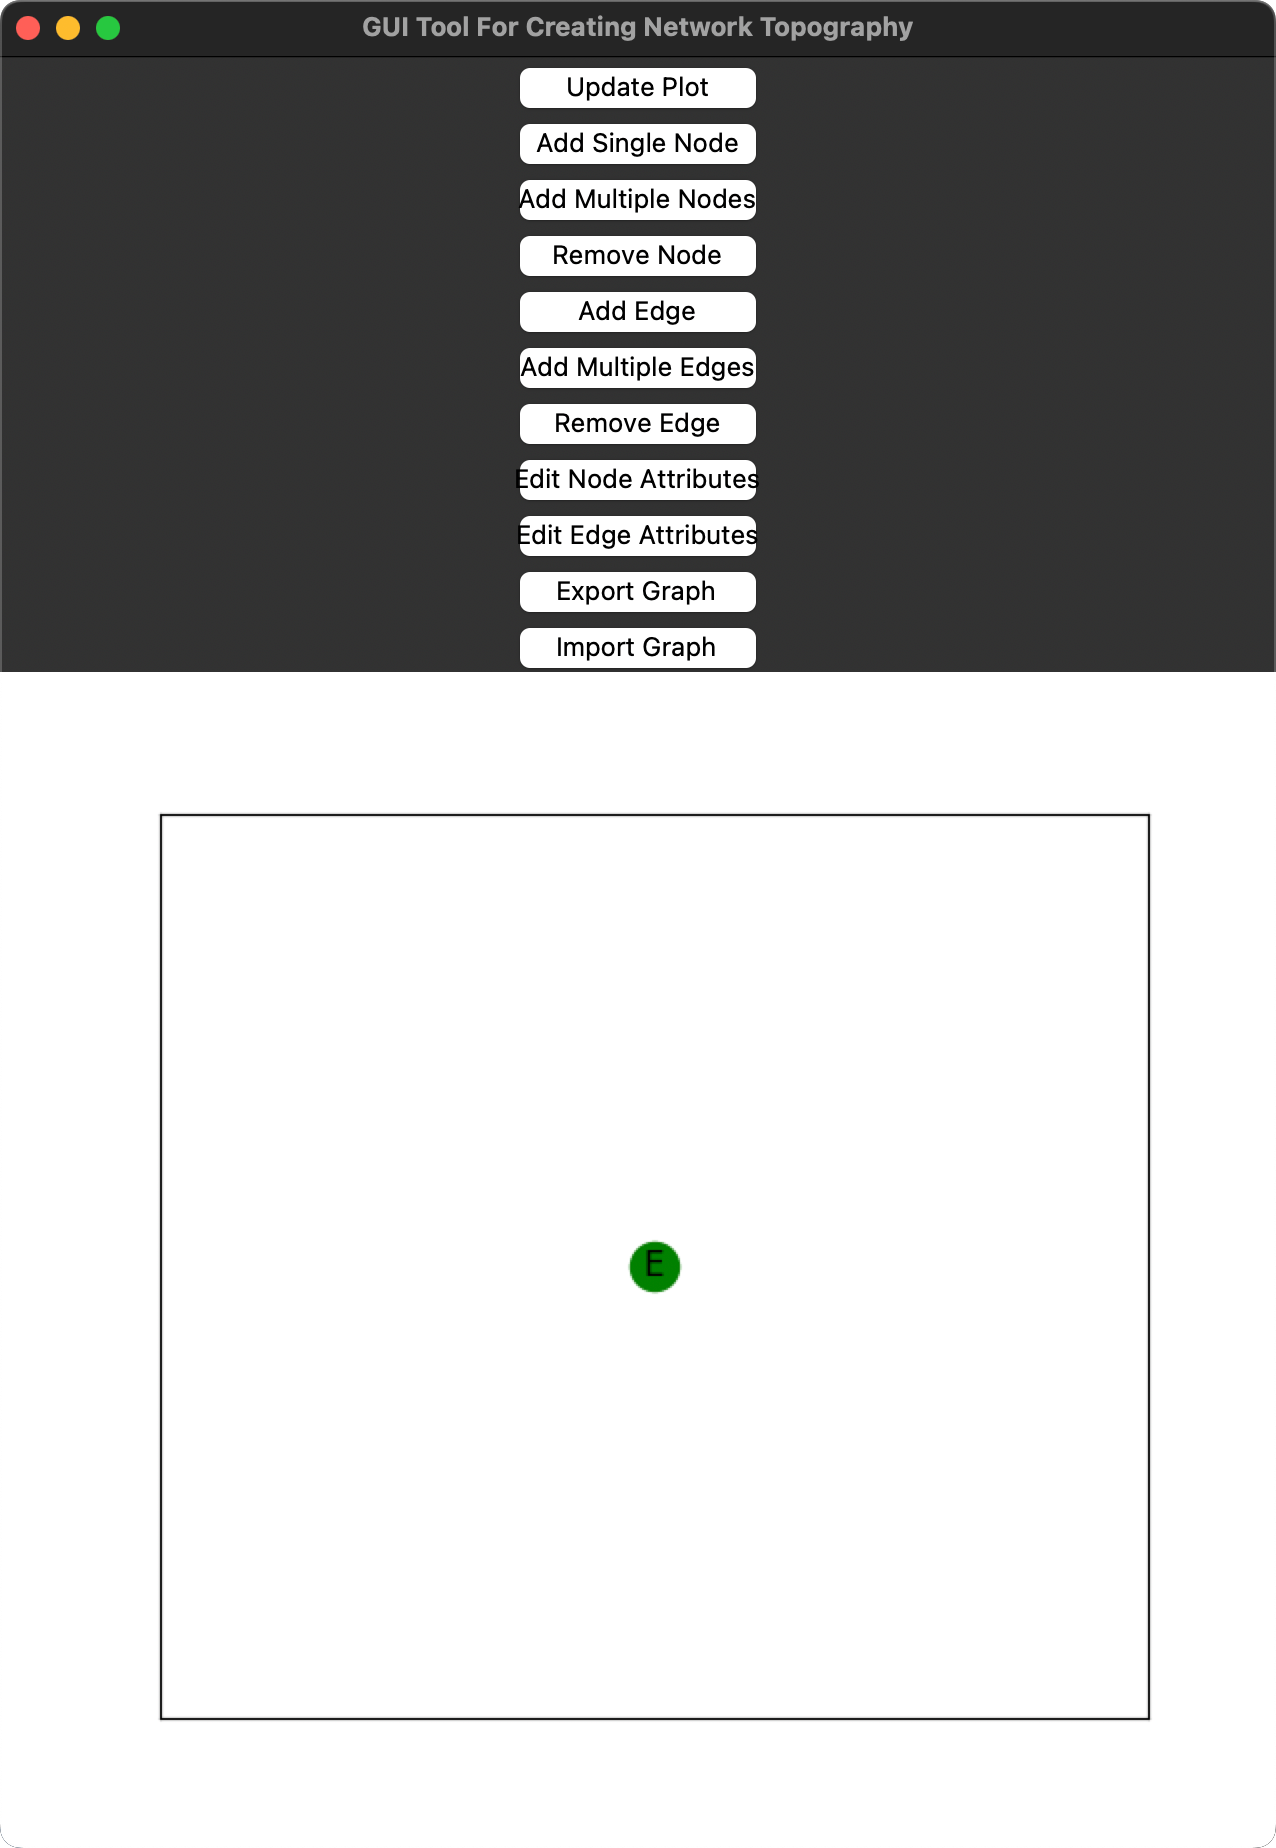
\includegraphics[width=\linewidth]{Screenshots/initial_startup_GUI_tool.png}
        \caption{
            The GUI tool as seen on the startup of the program.
        }
        \label{fig:ss:initial_startup_GUI_tool}
    \end{subfigure}
    \begin{subfigure}{0.49\linewidth}
        \centering
        \captionsetup{width=1\linewidth}
        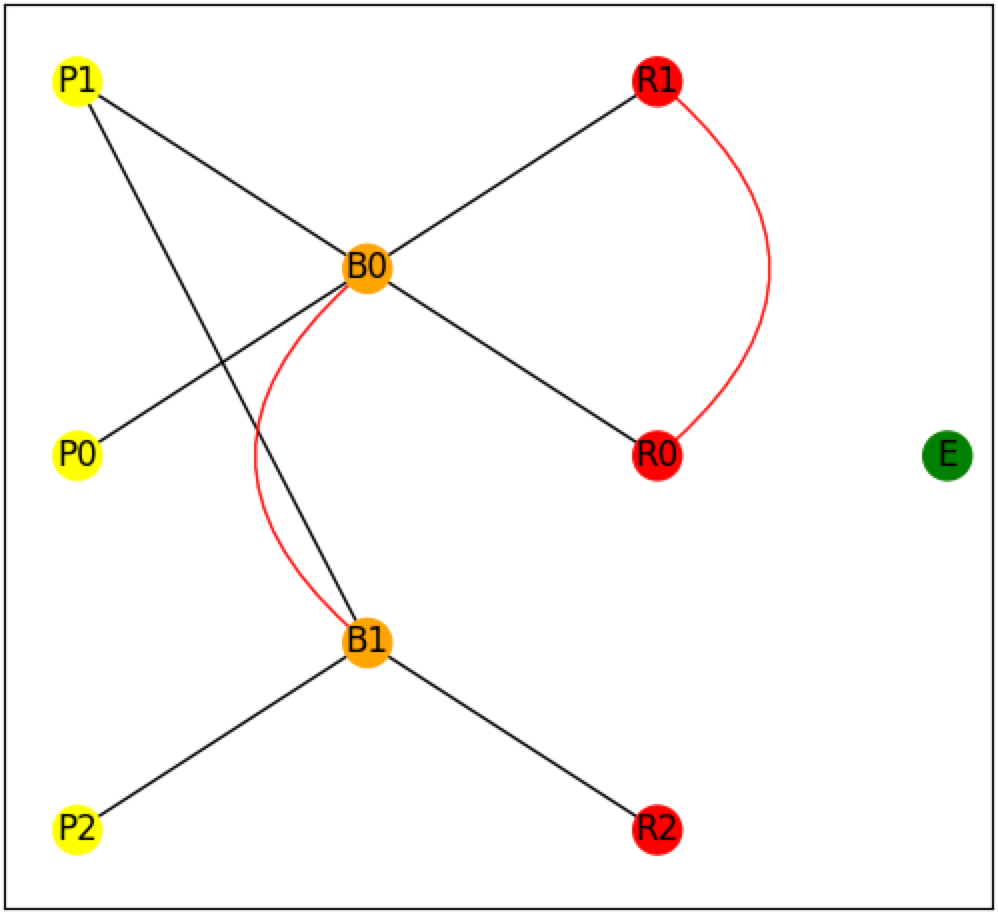
\includegraphics[width=\linewidth]{Screenshots/example_network.png}
        \caption{
            An arbitrary $3\times2\times3$ and $1\times 1 \times 1$ network with each node representing a phage, bacteria, or resource, with arbitrary interactions occurring between them. 
            Although not used here, edges between the same agent types and self loops are allowed. 
            This network topography along with a $1 \times 1 \times 1$ network will be used in the \nameref{Methods} and \nameref{AER} sections. 
        }
        \label{fig:ss:example_network}
    \end{subfigure} 
 \end{figure}

\subsection{Simulation Framework}
\label{sec:simulation_framework}
The user provides an ODE model and the network topography as input to the framework. 
The simulation framework deals with handling the input, output, collecting and storing of the simulation input and output.
The framework uses SciPy's \cite{virtanenSciPy10Fundamental2020} \textit{solve\_ivp()} numerical solver \cite{ dormandFamilyEmbeddedRungeKutta1980} to simulate the provided ODE equations and calculate the population levels through time.
The user receives two outputs from the framework. 
The first output is an array of time values that the solver used to calculate the population count.
The second output is an array containing the population count at each time step for every agent.

In order to facilitate more complex model behavior, "hidden" agents can be added to the simulation, where the hidden agents represent states that a "visible" agent can be in. 
Such an example would be the distinction between uninfected and infected bacteria. 
Each bacteria agent $b_i$ would contain two hidden sub-agents, called sub-agent states, an uninfected sub-agent state $b_{i_\text{uninfected}}$ and infected sub-agent state $b_{i_\text{infected}}$. 
It is possible to create further sub-agents, by having a bacteria go through $M$ stages of infection. 
So each infected agent has sub-agent $b_{i_{\text{infected}_k}}$, where $1 \leq k \leq M$. 

In the network model you would explicitly create a $3\times 2 \times 3$ network, but when passing the network to the simulation framework, you would tell the framework to model the subagents. 
The user's ODE model has to correctly model each (hidden) agent and correctly handle the changes in states. 

Even though the user might submit a $3 \times 2 \times 3$ model, if the user follows the uninfected and infected classification, where each bacterium goes through $4$ stages, the ODE model and framework will explicitly be modelling 3 phages, 10 bacteria (2 uninfected + $2\cdot 4=10$ infected bacteria), and 3 resources. 

The user might also be interested in modelling a resource reservoir in a chemostat, where resources go from an external reservoir not accessible by the bacteria to the virtual chemostat ready to be consumed by the bacteria. 
3 hidden resource agents would be added to the system, where the resources would model the transfer of resources from the reservoir to the simulation environment. 
The provided ODE model will have to correctly model and transfer the resources from $R_{i_{\text{reservoir}}}$ to $R_{j_{\text{chemostat}}}$. 

\subsection{Visualization Dashboard}
\label{sec:visualization_framework}
The third part involves analyzing and visualizing the simulation results on an interactive Dash Plotly \cite{DashDocumentationUser} dashboard. 
The user can use a dashboard built using Plotly Dash to interact with the solver and network.
The user can interact with the solver and network by changing parameter, environment, and setting values on the fly.
This allows the user to quickly change parameter values and test different situations.
The dashboard includes various starter plots that allow the user to test the model.
As output, the dashboard will show interactive plots so that the user can analyze the system. 


The dashboard allows the user to interact with the network, the model, and some prebuilt visualizations, and is built into three logical sections.
The first section allows for the user to edit the network parameters and setting values on the fly to quickly iterate through different conditions and to fine-tune parameter selection without having to rebuild the network using the GUI tool.
The second section allows for the user to see how the population count evolves over time for a given initial condition and parameter values, allowing to quickly test the network input.
The final section allows for the user to run more advanced analyses on the network, for example, by changing multiple parameter values and visualizing the output. 

\subsubsection{Editing Network and Parameter Values}
\label{sec:editing_network_and_parameter_values}
The editing network and parameter value contain five separate sections.
\paragraph{Initial Condition}
The initial condition settings panel (\Cref{fig:ss:ds:initial_condition}) allows for the user to edit the initial starting values of the agents. 
Each agent type has a table containing the initial population count. 
Extra hidden agents can be included. 
When a bacteria has been infected, the bacteria goes through multiple stages before lysing. Each bacteria agent starts out as uninfected, and once infected, the bacteria goes through 4 stages of infection before lysing as seen in \Cref{fig:ss:ds:initial_condition}.  
\paragraph{Vector Data} 
Data that can be represented as a vector, for example the data attributed to an agent type have their own section, \Cref{fig:ss:ds:vector}.
\paragraph{Matrix Data}
Data that is stored as a matrix, the data stored on edges between agents, is stored in the matrix tab (\Cref{fig:ss:ds:matrix}).
\paragraph{Environment and settings}
The environment data and settings data also have their own tab, \Cref{fig:ss:ds:environment} and \Cref{fig:ss:ds:settings} respectively.

\begin{figure}[!ht]
    \centering
    \begin{subfigure}{0.49\linewidth}
        \centering
        \captionsetup{width=1\linewidth}
        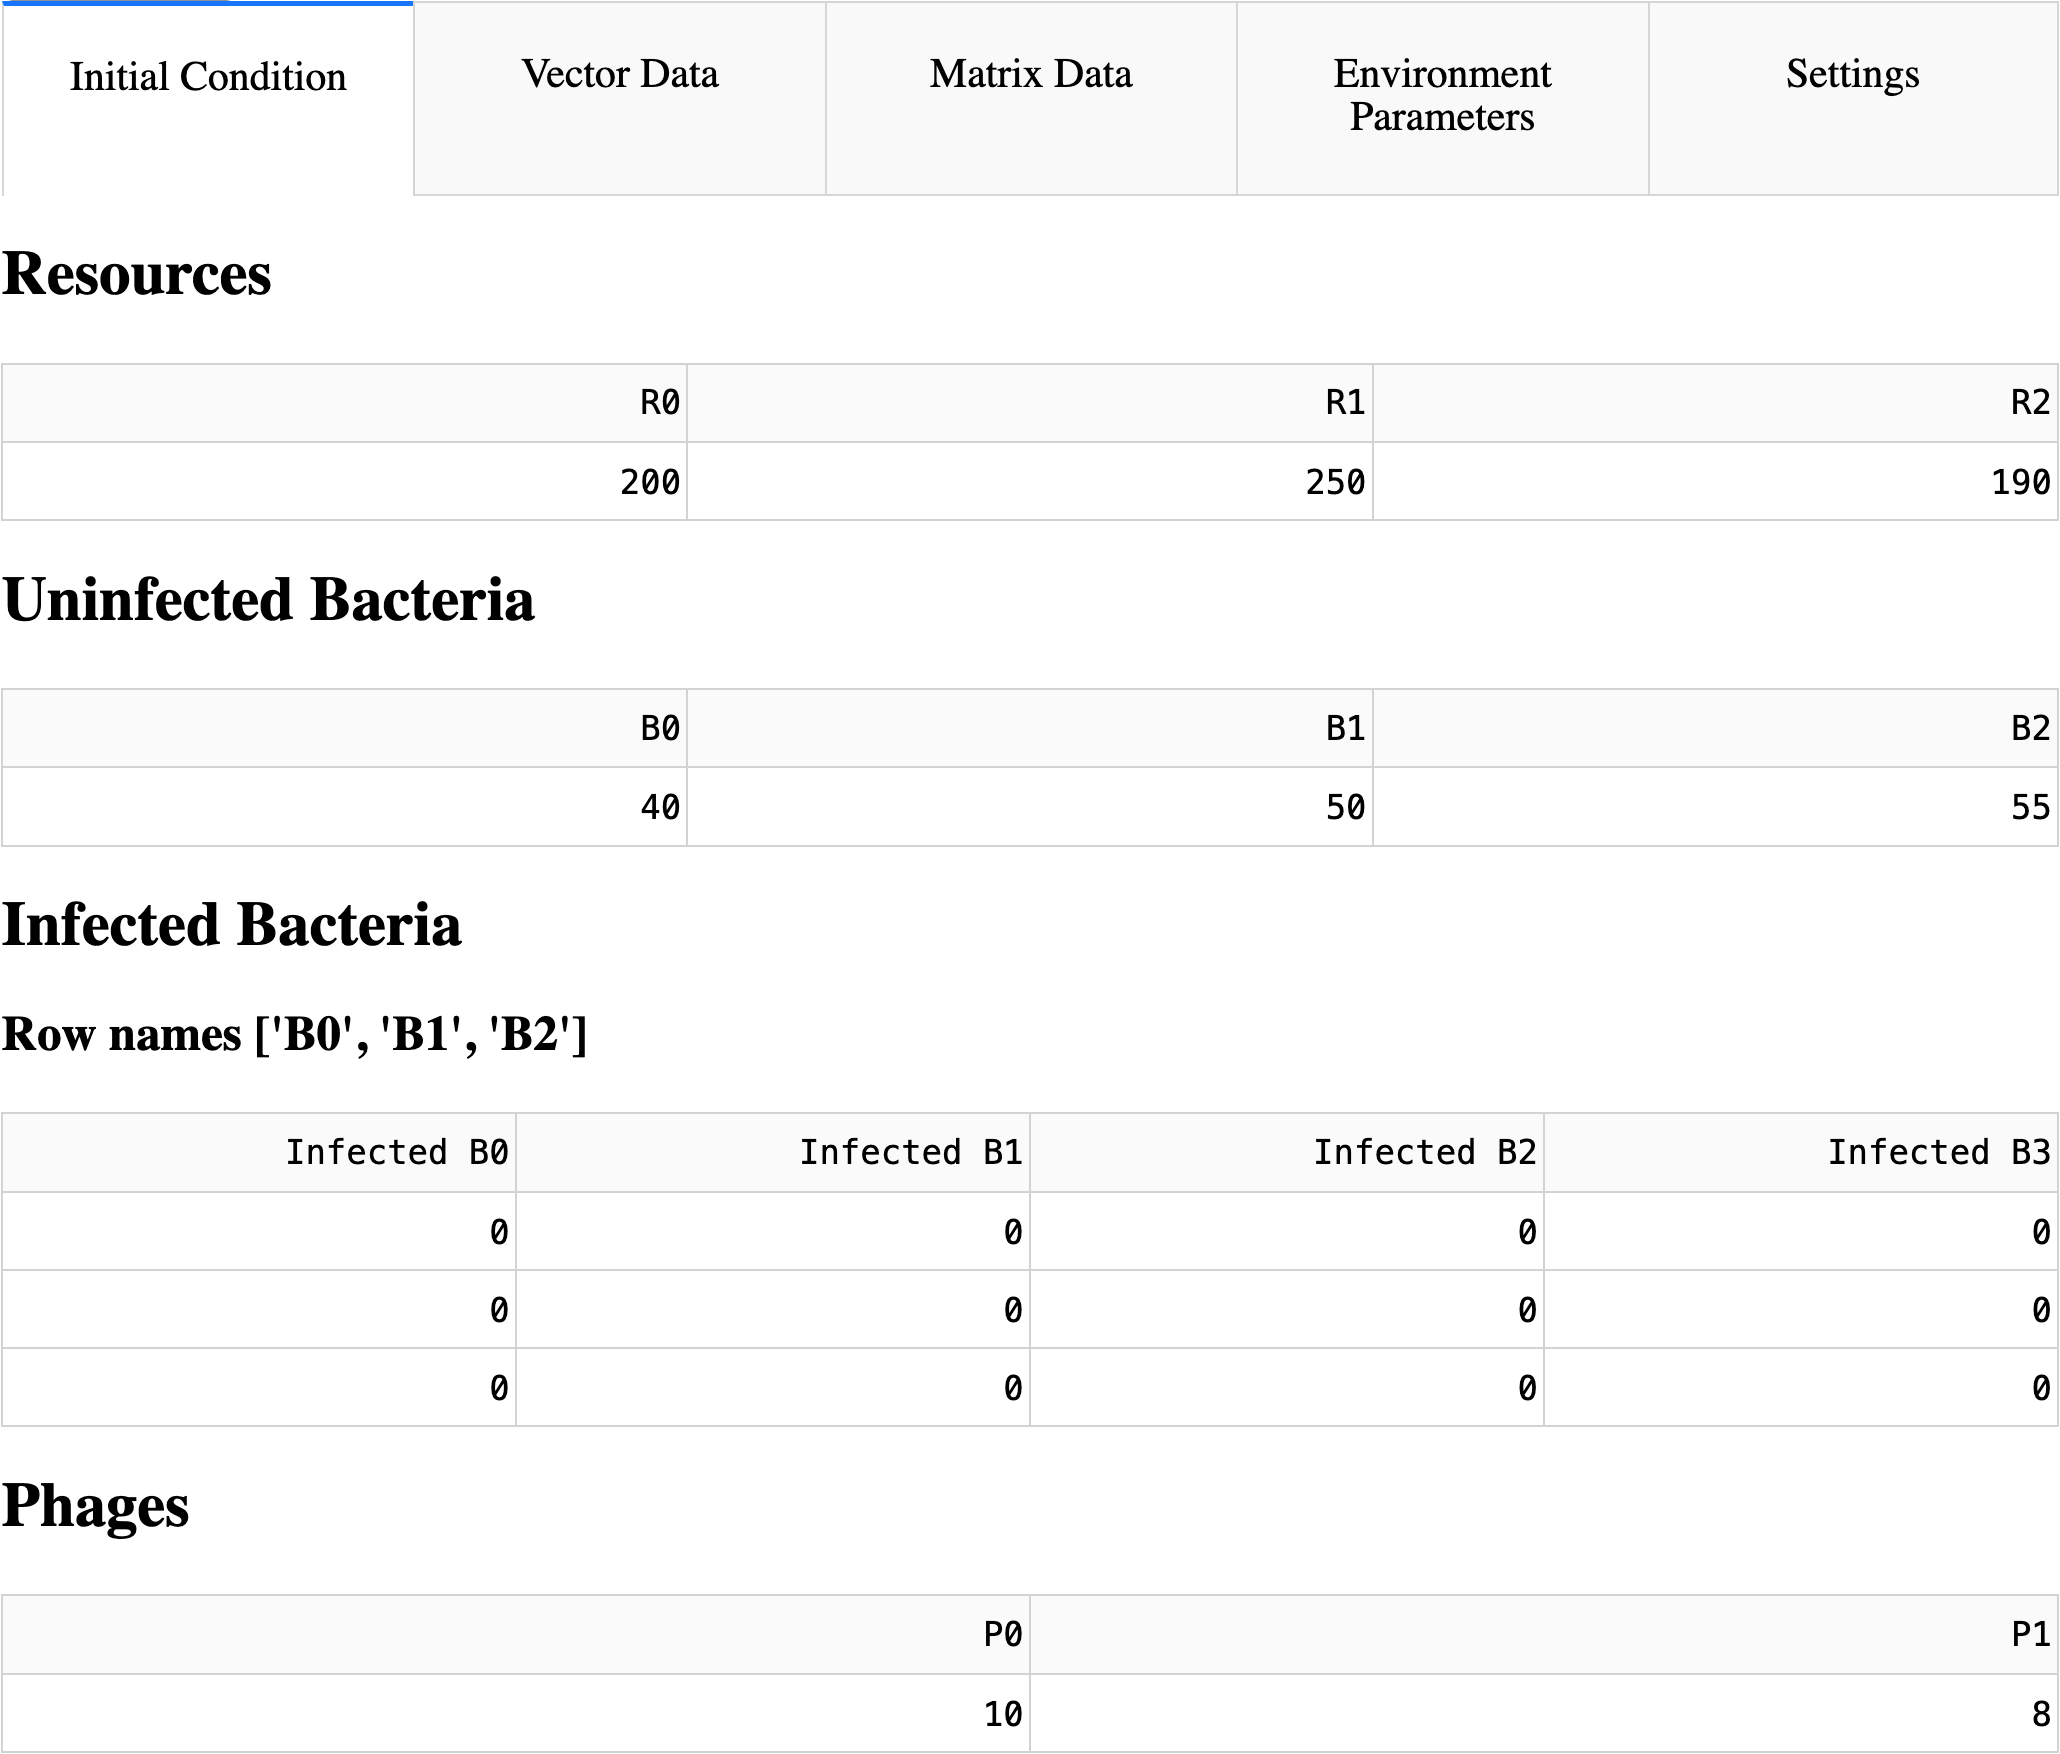
\includegraphics[width=\linewidth]{Screenshots/DashboardSettings/initial_condition_settings.png}
        \caption{
            The tab where the user can edit the initial conditions of the agents.
        }
        \label{fig:ss:ds:initial_condition}
    \end{subfigure}
    \hfill
    \begin{subfigure}{0.49\linewidth}
        \centering
        \captionsetup{width=1\linewidth}
        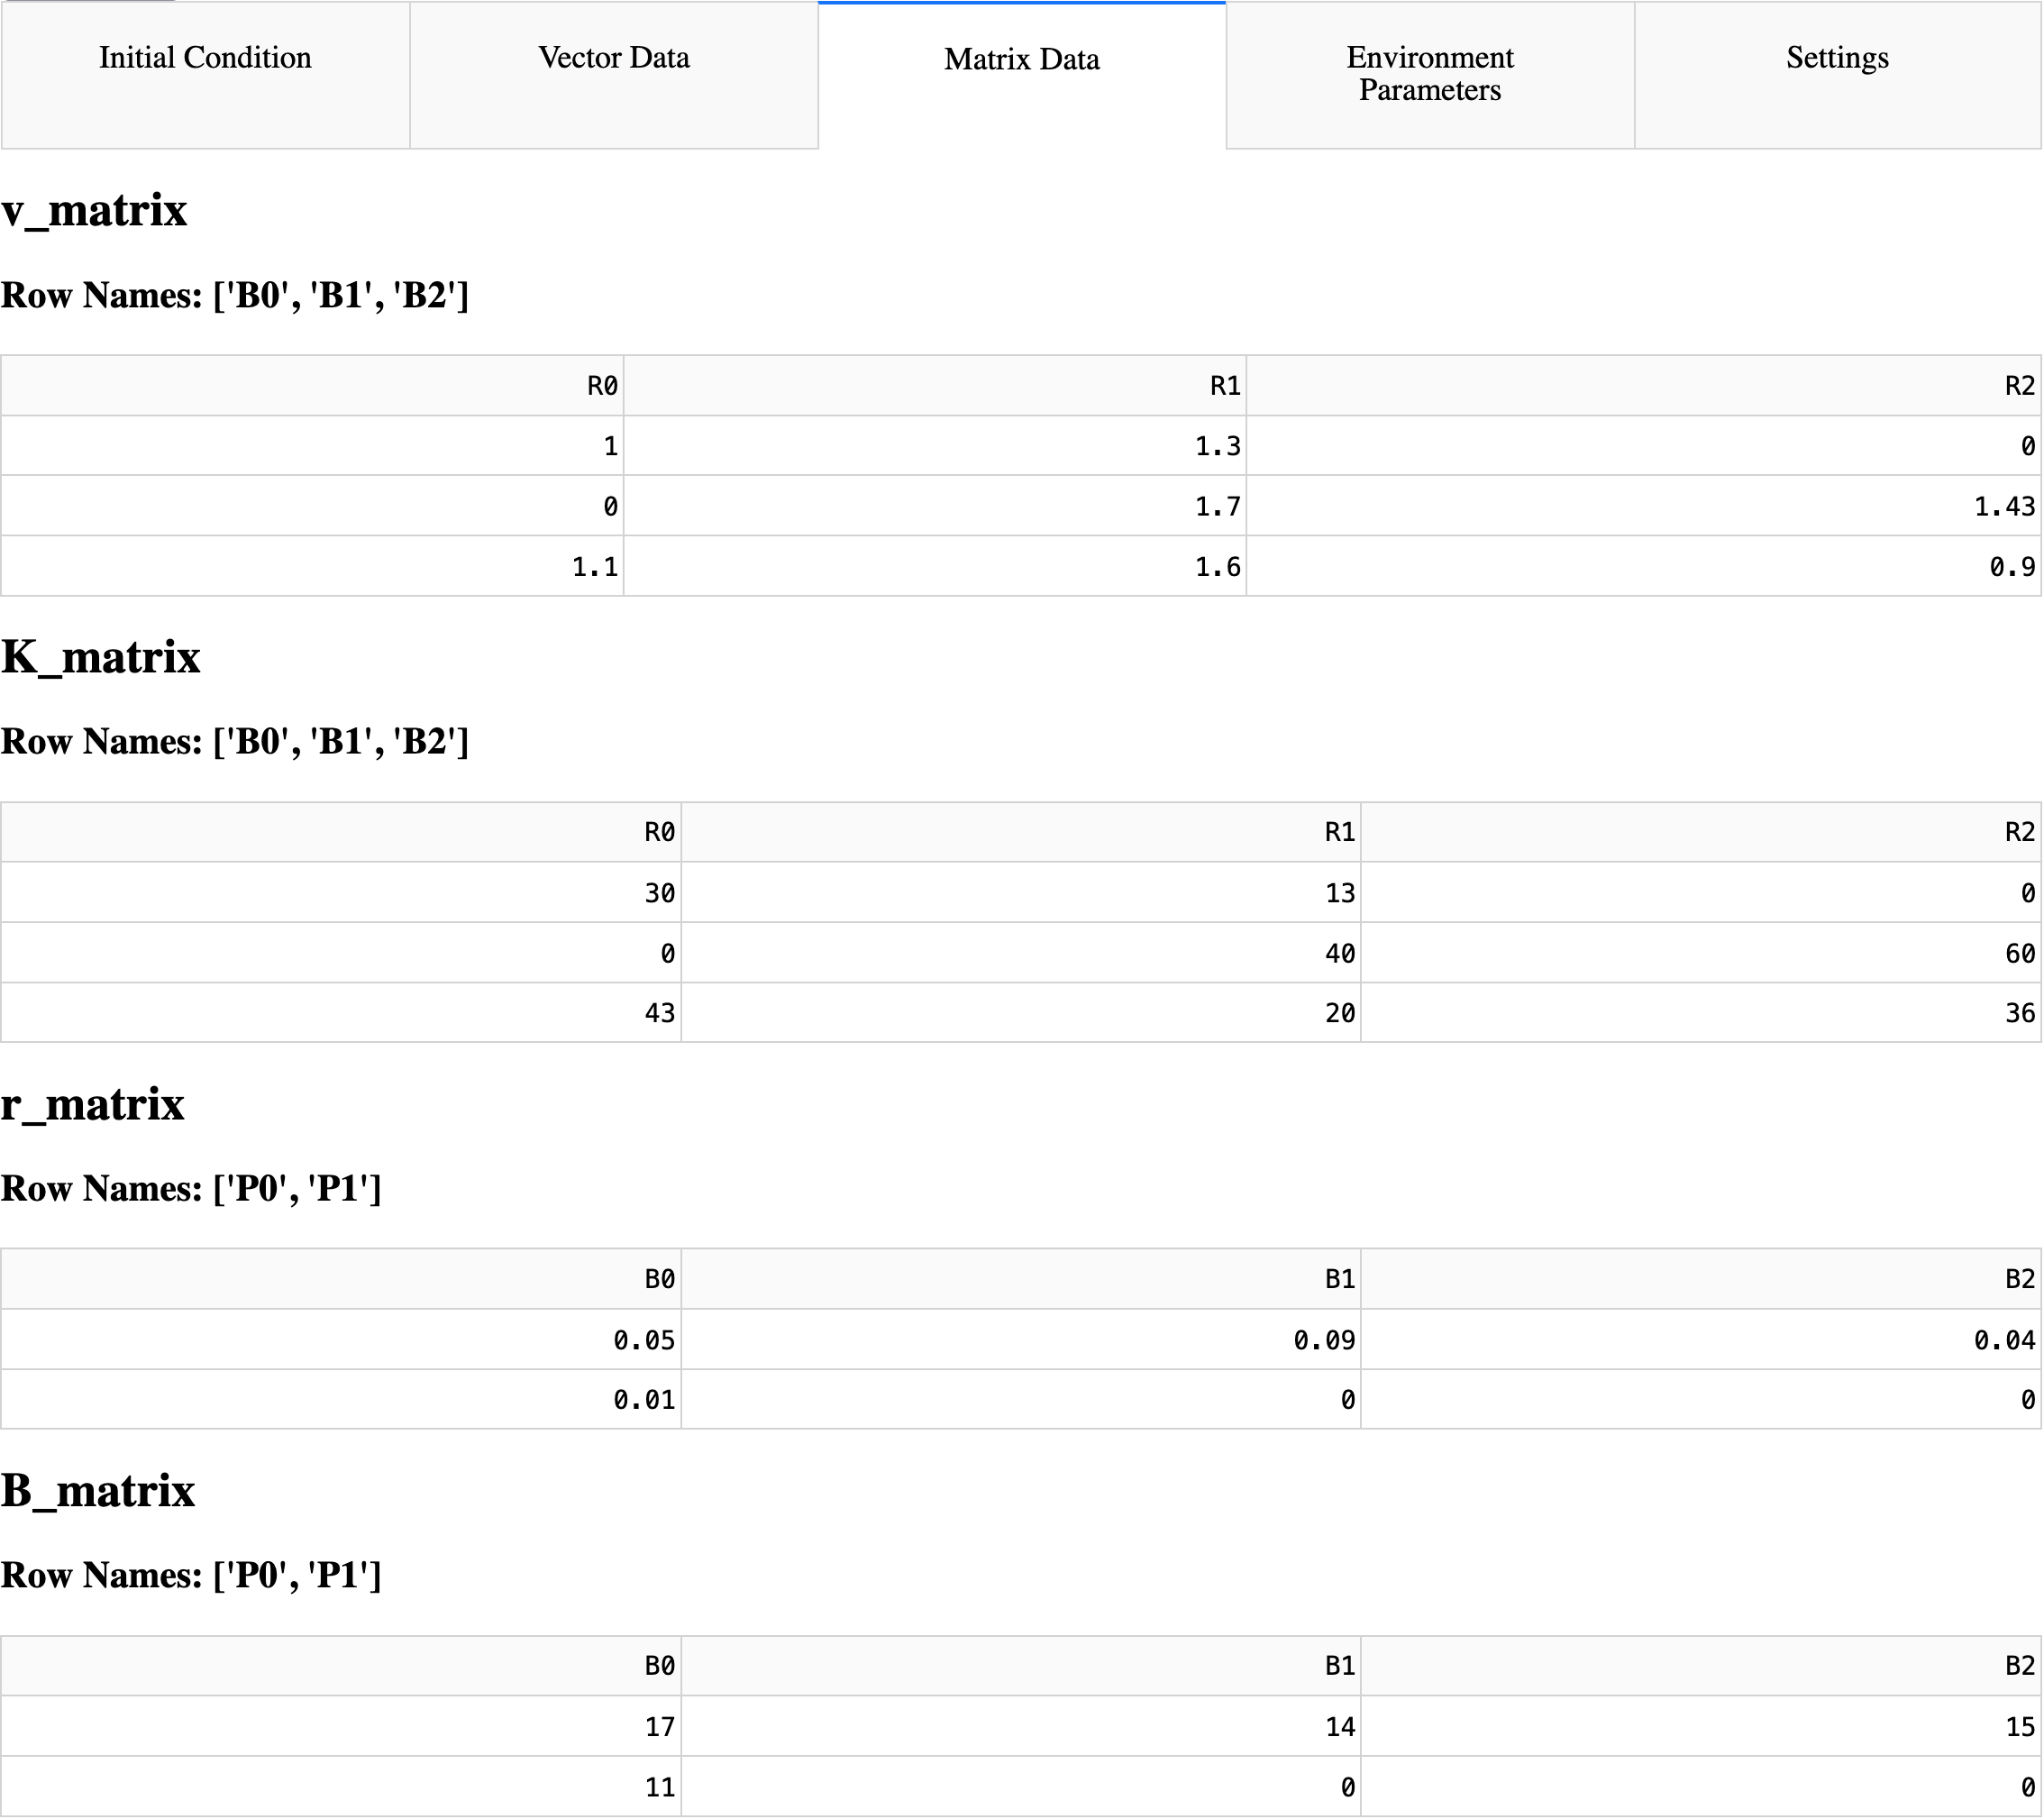
\includegraphics[width=\linewidth]{Screenshots/DashboardSettings/initial_matrix_settings.png}
        \caption{
            The tab where the user can edit the matrix attribute values. 
        }
        \label{fig:ss:ds:matrix}
    \end{subfigure}
    \hfill
    \begin{subfigure}{0.49\linewidth}
        \centering
        \captionsetup{width=1\linewidth}
        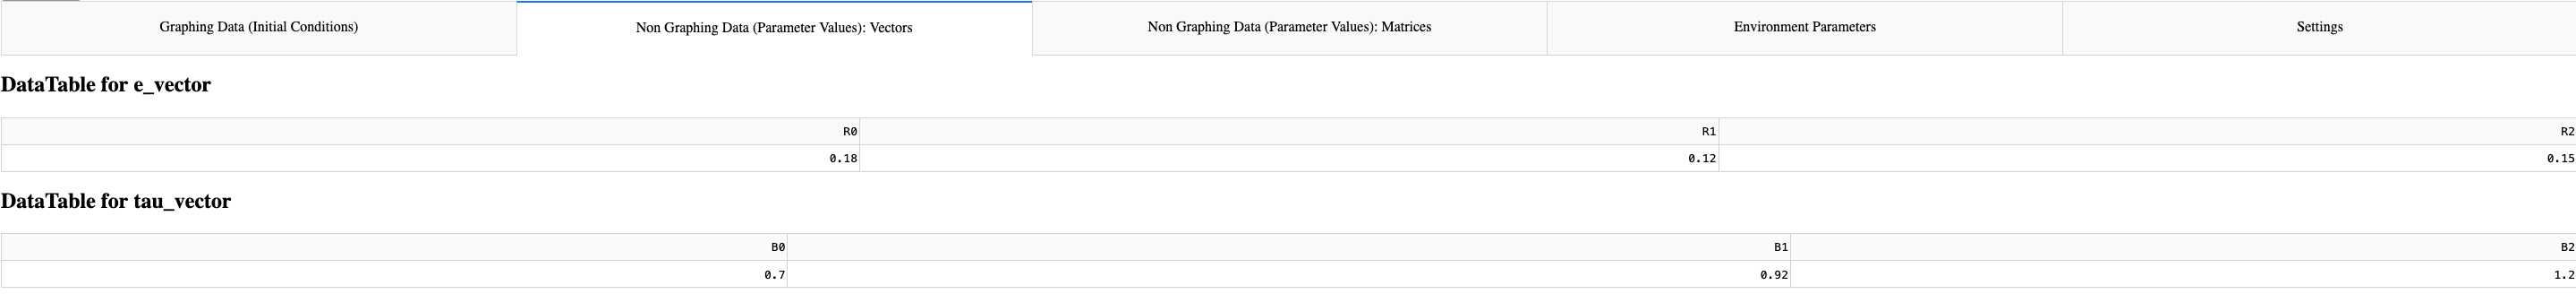
\includegraphics[width=\linewidth]{Screenshots/DashboardSettings/initial_vector_settings.png}
        \caption{
            The tab where the user can edit the vector attribute values.
        }
        \label{fig:ss:ds:vector}
    \end{subfigure}
    \hfill
    \begin{subfigure}{0.49\linewidth}
        \centering
        \captionsetup{width=1\linewidth}
        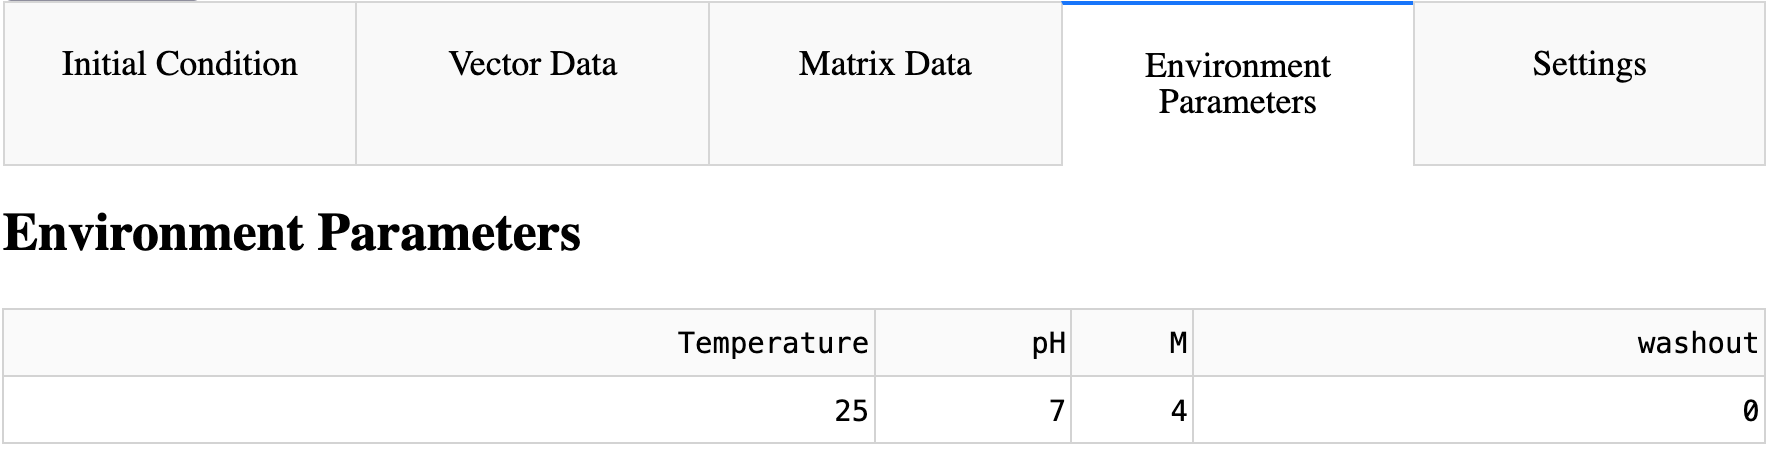
\includegraphics[width=\linewidth]{Screenshots/DashboardSettings/initial_environment_settings.png}
        \caption{
            The tab where the user can edit the environment values. 
        }
        \label{fig:ss:ds:environment}
    \end{subfigure}
    \hfill
    \begin{subfigure}{0.49\linewidth}
        \centering
        \captionsetup{width=1\linewidth}
        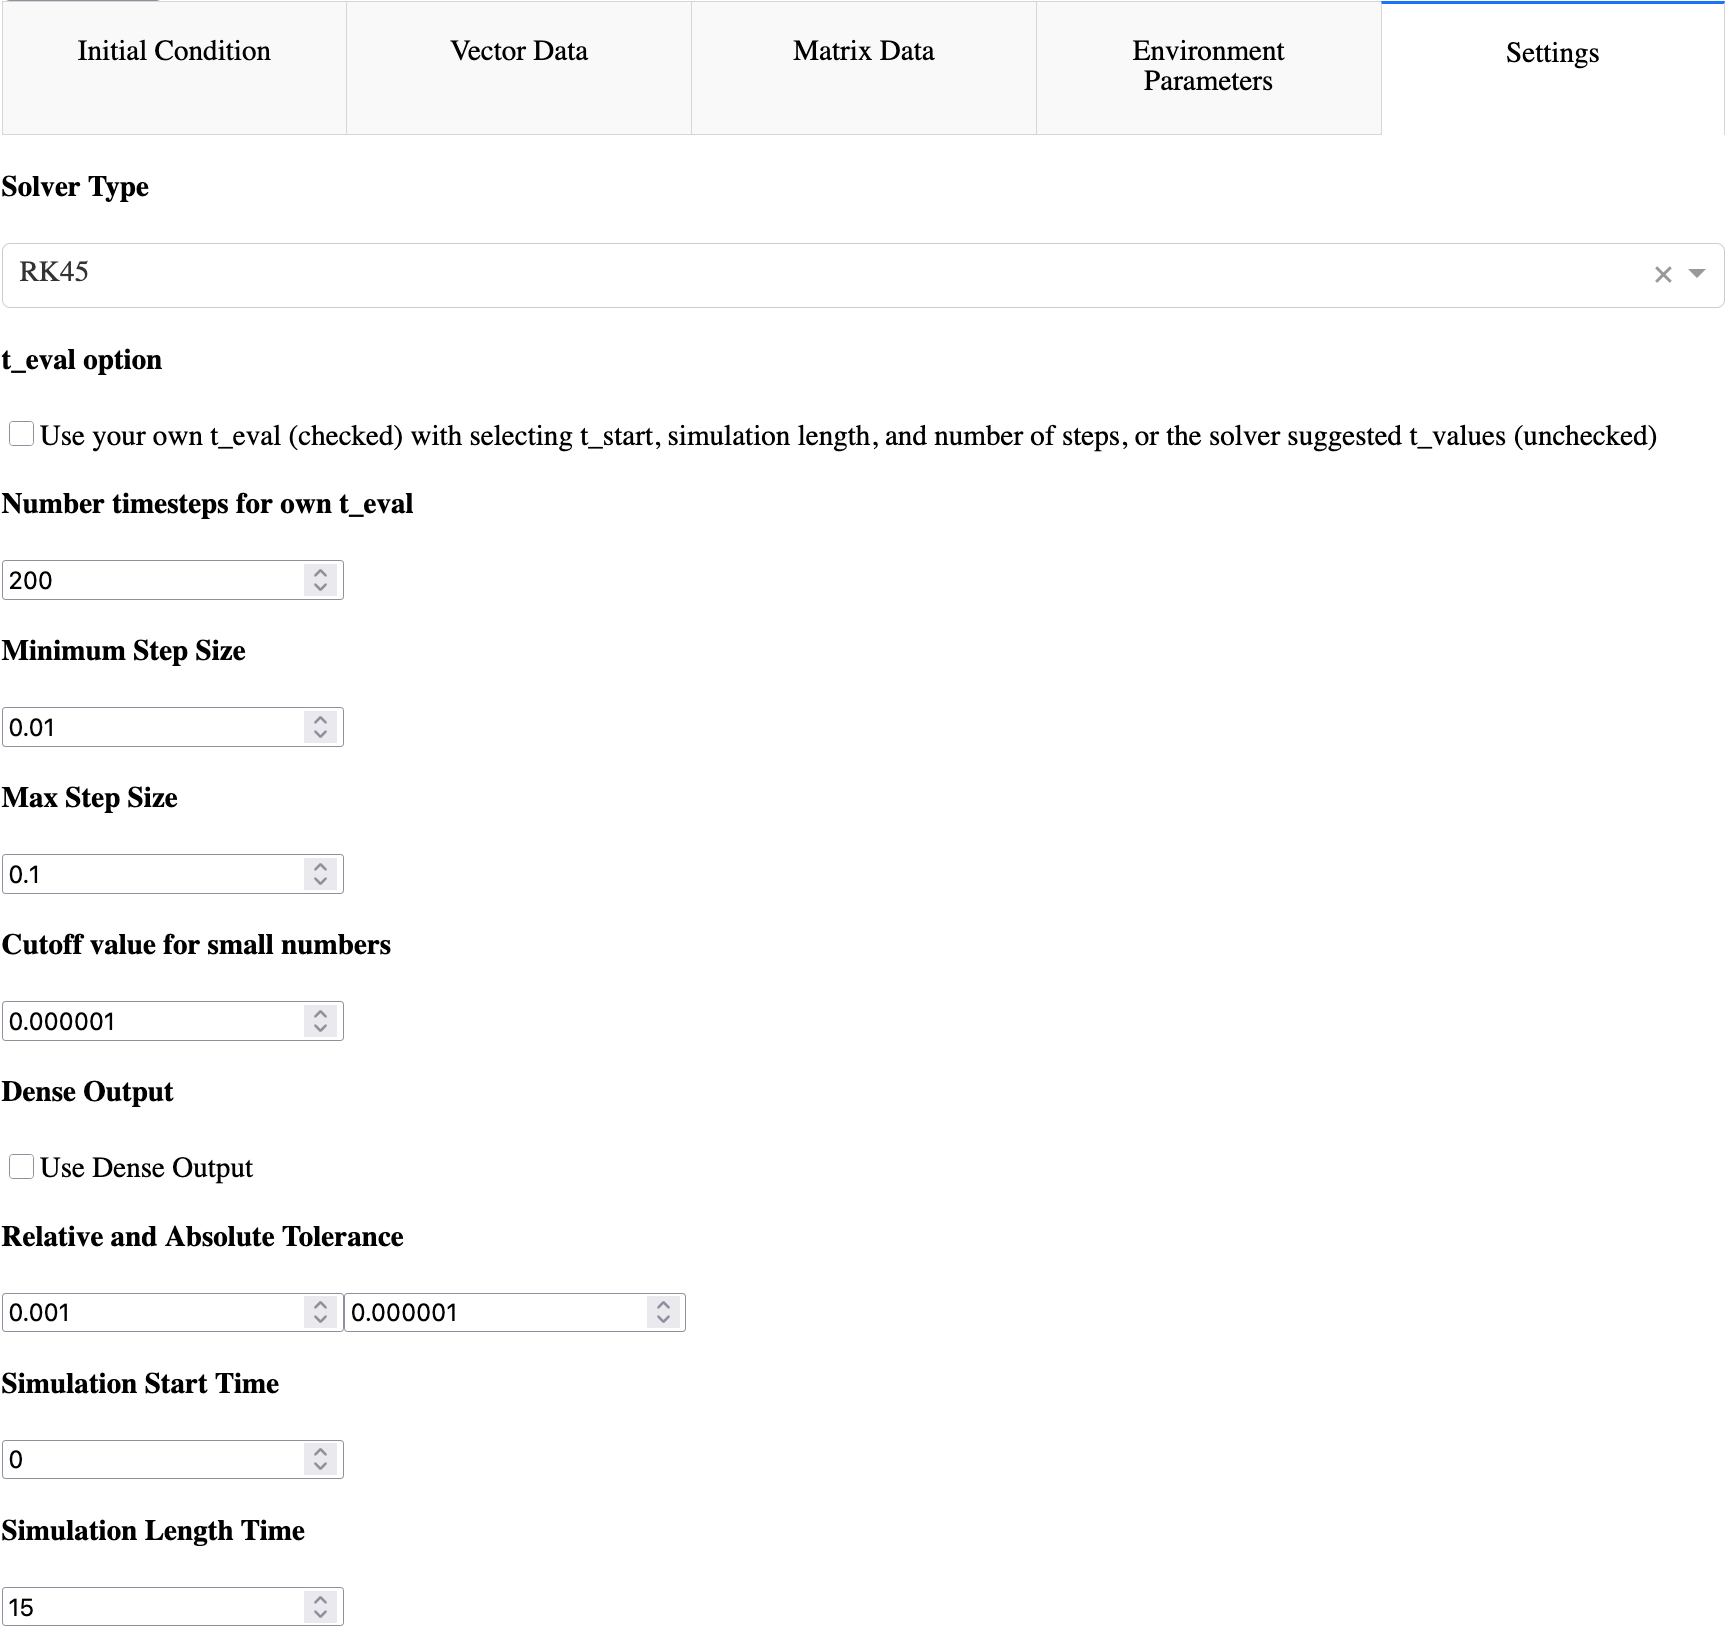
\includegraphics[width=\linewidth]{Screenshots/DashboardSettings/initial_settings_settings.png}
        \caption{
            The tab where a user can edit the settings of the solver and simulation. 
        }
        \label{fig:ss:ds:settings}
    \end{subfigure}
    \caption{The tabs where the user can edit the various parameter values and control the simulation parameters}
 \end{figure}

\subsubsection{Visualization and Analysis}
In the analysis section, the user can run different analysis methods to gain a greater understanding of the model.
For simplicity, the visualizations only support a $1 \times 1\times 1$ model, in order to make the analysis easier for the user, and to make it easier to analyze the visualization as the aim of the tool is to gain a deeper understanding of the interactions in a reduced complexity environment. 
These advanced visualizations were created with the mind of understanding a simple network.
There are five different analysis and visualization methods, and one system where the user can run a large simulation on the whole network and receive an output file containing the raw simulation file data.
The raw data is stored as a \textit{parquet} file, a tabular-like data format, which when combined with Dask \cite{DaskDaskDocumentation}, allows for querying of the data similarly to Pandas.
Parquet with Dask offers superior performance and data storage solutions that Pandas can't offer.
Once queried, the user can create their own graphs and plots as they have access to the parameter values used and the raw simulation data.

\paragraph{Serial Transfer}
\label{sec:serial_transfer}
Serial transfer is a method employed by bacteriologist where after a set amount of time, the bacteriologist pipettes a specified amount of media (for example 10ml of liquid) containing bacteria and resources, possibly with phages, and transfers the old media into a solution containing new media.
At this stage, the bacteriologist can introduce new agents, or re-introduce agents if the agent population or concentration has died out.
However, usually only resources are added during the transfer process.
An example would be an experiment starts with 50ml of solution.
The experiment runs for 24 hours before 5ml is removed.
Researchers can run various tests, such as using optical density measurements to assess bacterial density in the solution or employing a mass spectrometer to determine the concentration of the resources.
The 5ml is then re-added to a new solution of 45ml containing fresh resources.
The effect that this has is it creates a sort of artificial stable point.
As the bacteria grow, they consume the resources found in the solution.
However eventually the resources run out, and the bacteria die out due to a lack of resources.
By introducing new resources at set time intervals, the bacteria can regrow and exhibit a semi-stationary behavior.

The implementation of serial transfer is slightly different.
A user can select a number which will divide the population count of the agents by that number (\Cref{fig:ss:av:serial_transfer_settings}).
Then the program takes the initial condition values defined for the resources the initial condition in \Cref{sec:editing_network_and_parameter_values} and adds those values to the resources respectively.
By selecting a checkbox, the values as defined in the initial condition box for phages and bacteria in \Cref{sec:editing_network_and_parameter_values} can optionally be added as well.
As an example, if at the end of a simulation, there are 120 resources, 5000 bacteria, and 1000 phages remaining and the chosen serial transfer value is 15, then the resource, bacteria, and phage values would be decreased to 8, 333.33, and 66.66 respectively.
Then, if the initial condition for the resources, bacteria, and phages in \Cref{sec:editing_network_and_parameter_values} are 500, 80, and 10 respectively, and the checkbox is unchecked, the new population count will be 508, 333.33 and 66.66 respectively.
If the checkbox is checked, the new population count will be 508, 413.33, and 76.66 respectively.
These new values would be used as the new starting initial condition for a new simulation, and the run results will be appended to the previous run.
As output, new graphs are created showing the runs appended to one another, with an example output shown in \Cref{fig:ss:av:serial_transfer_run}.

\begin{figure}[!ht]
    \centering
    \begin{subfigure}{0.49\linewidth}
        \centering
        \captionsetup{width=1\linewidth}
        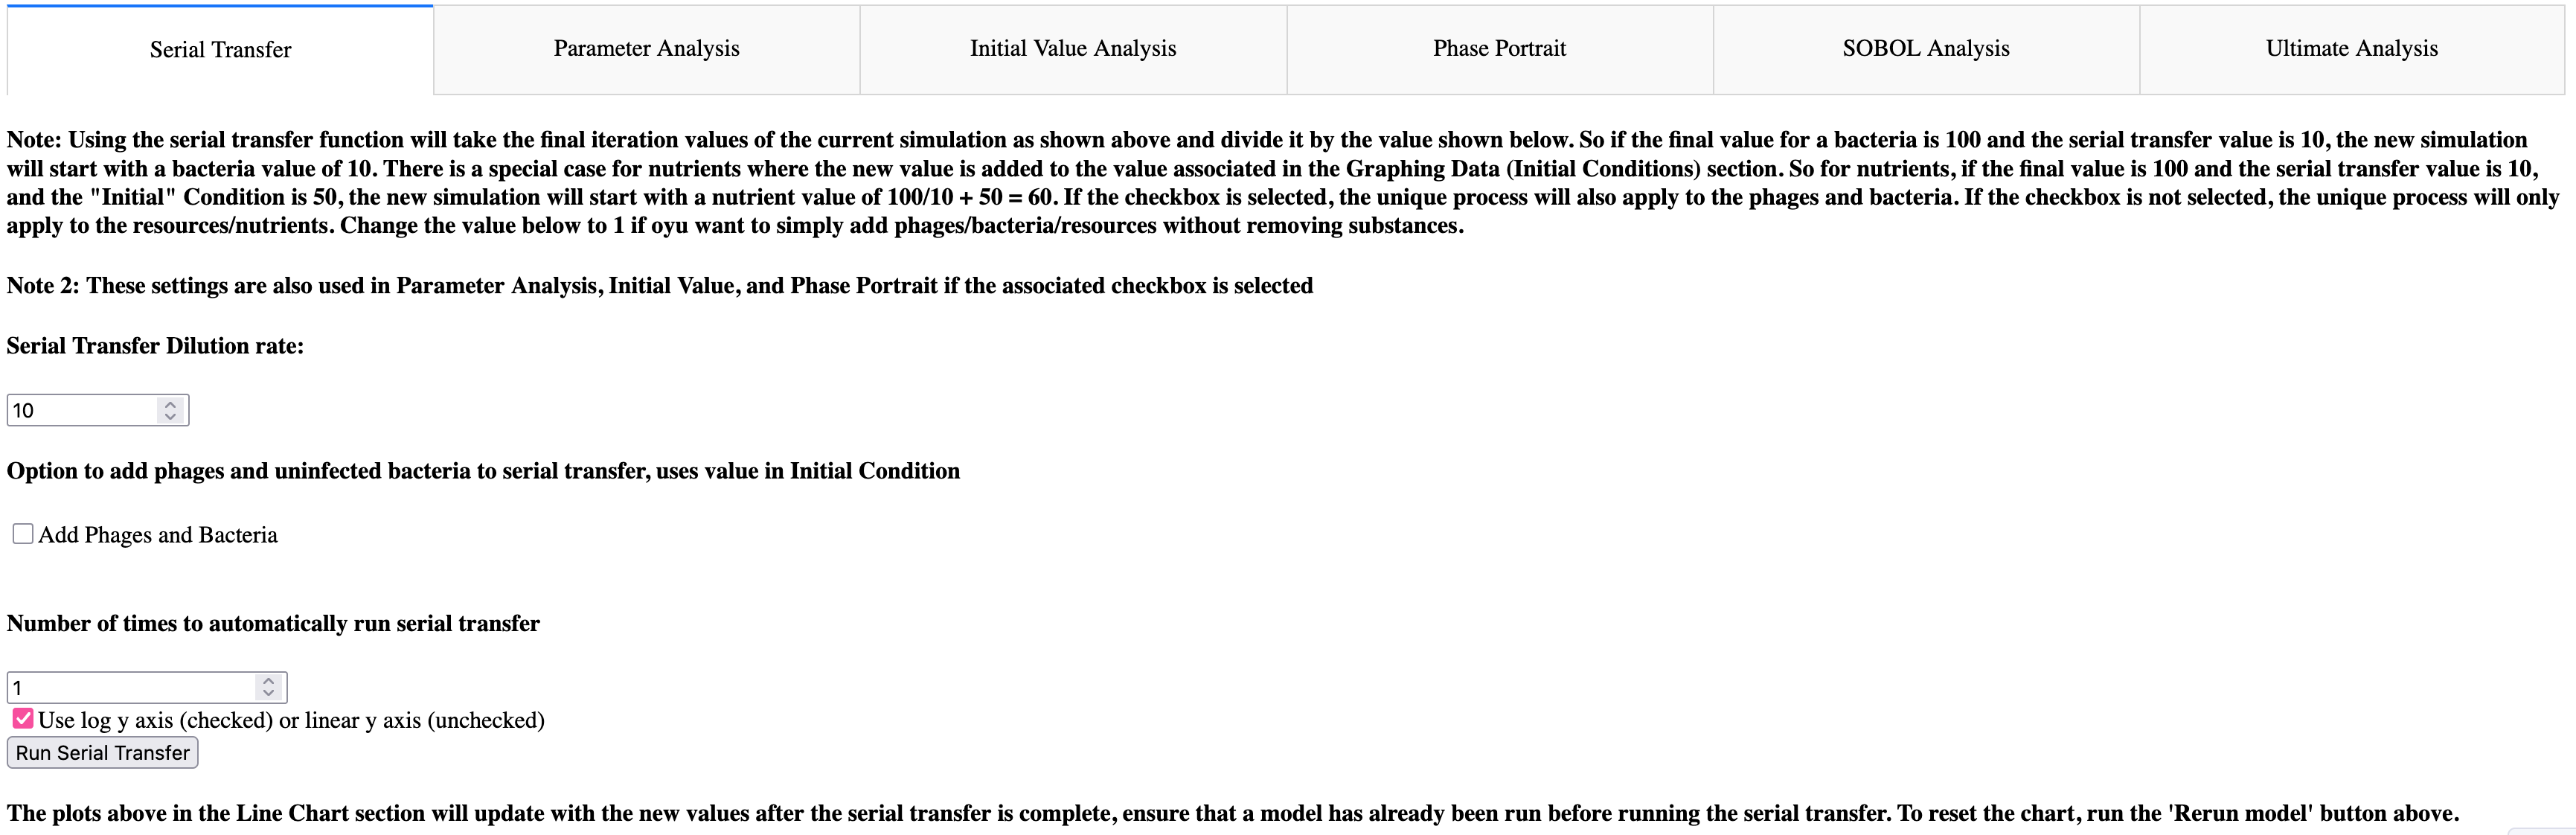
\includegraphics[width=\linewidth]{Screenshots/AdvancedVisualization/serial_transfer_settings.png}
        \caption{
            The section where the user can set up the serial transfer.
        }
        \label{fig:ss:av:serial_transfer_settings}
    \end{subfigure}
    \hfill
    \begin{subfigure}{0.49\linewidth}
        \centering
        \captionsetup{width=1\linewidth}
        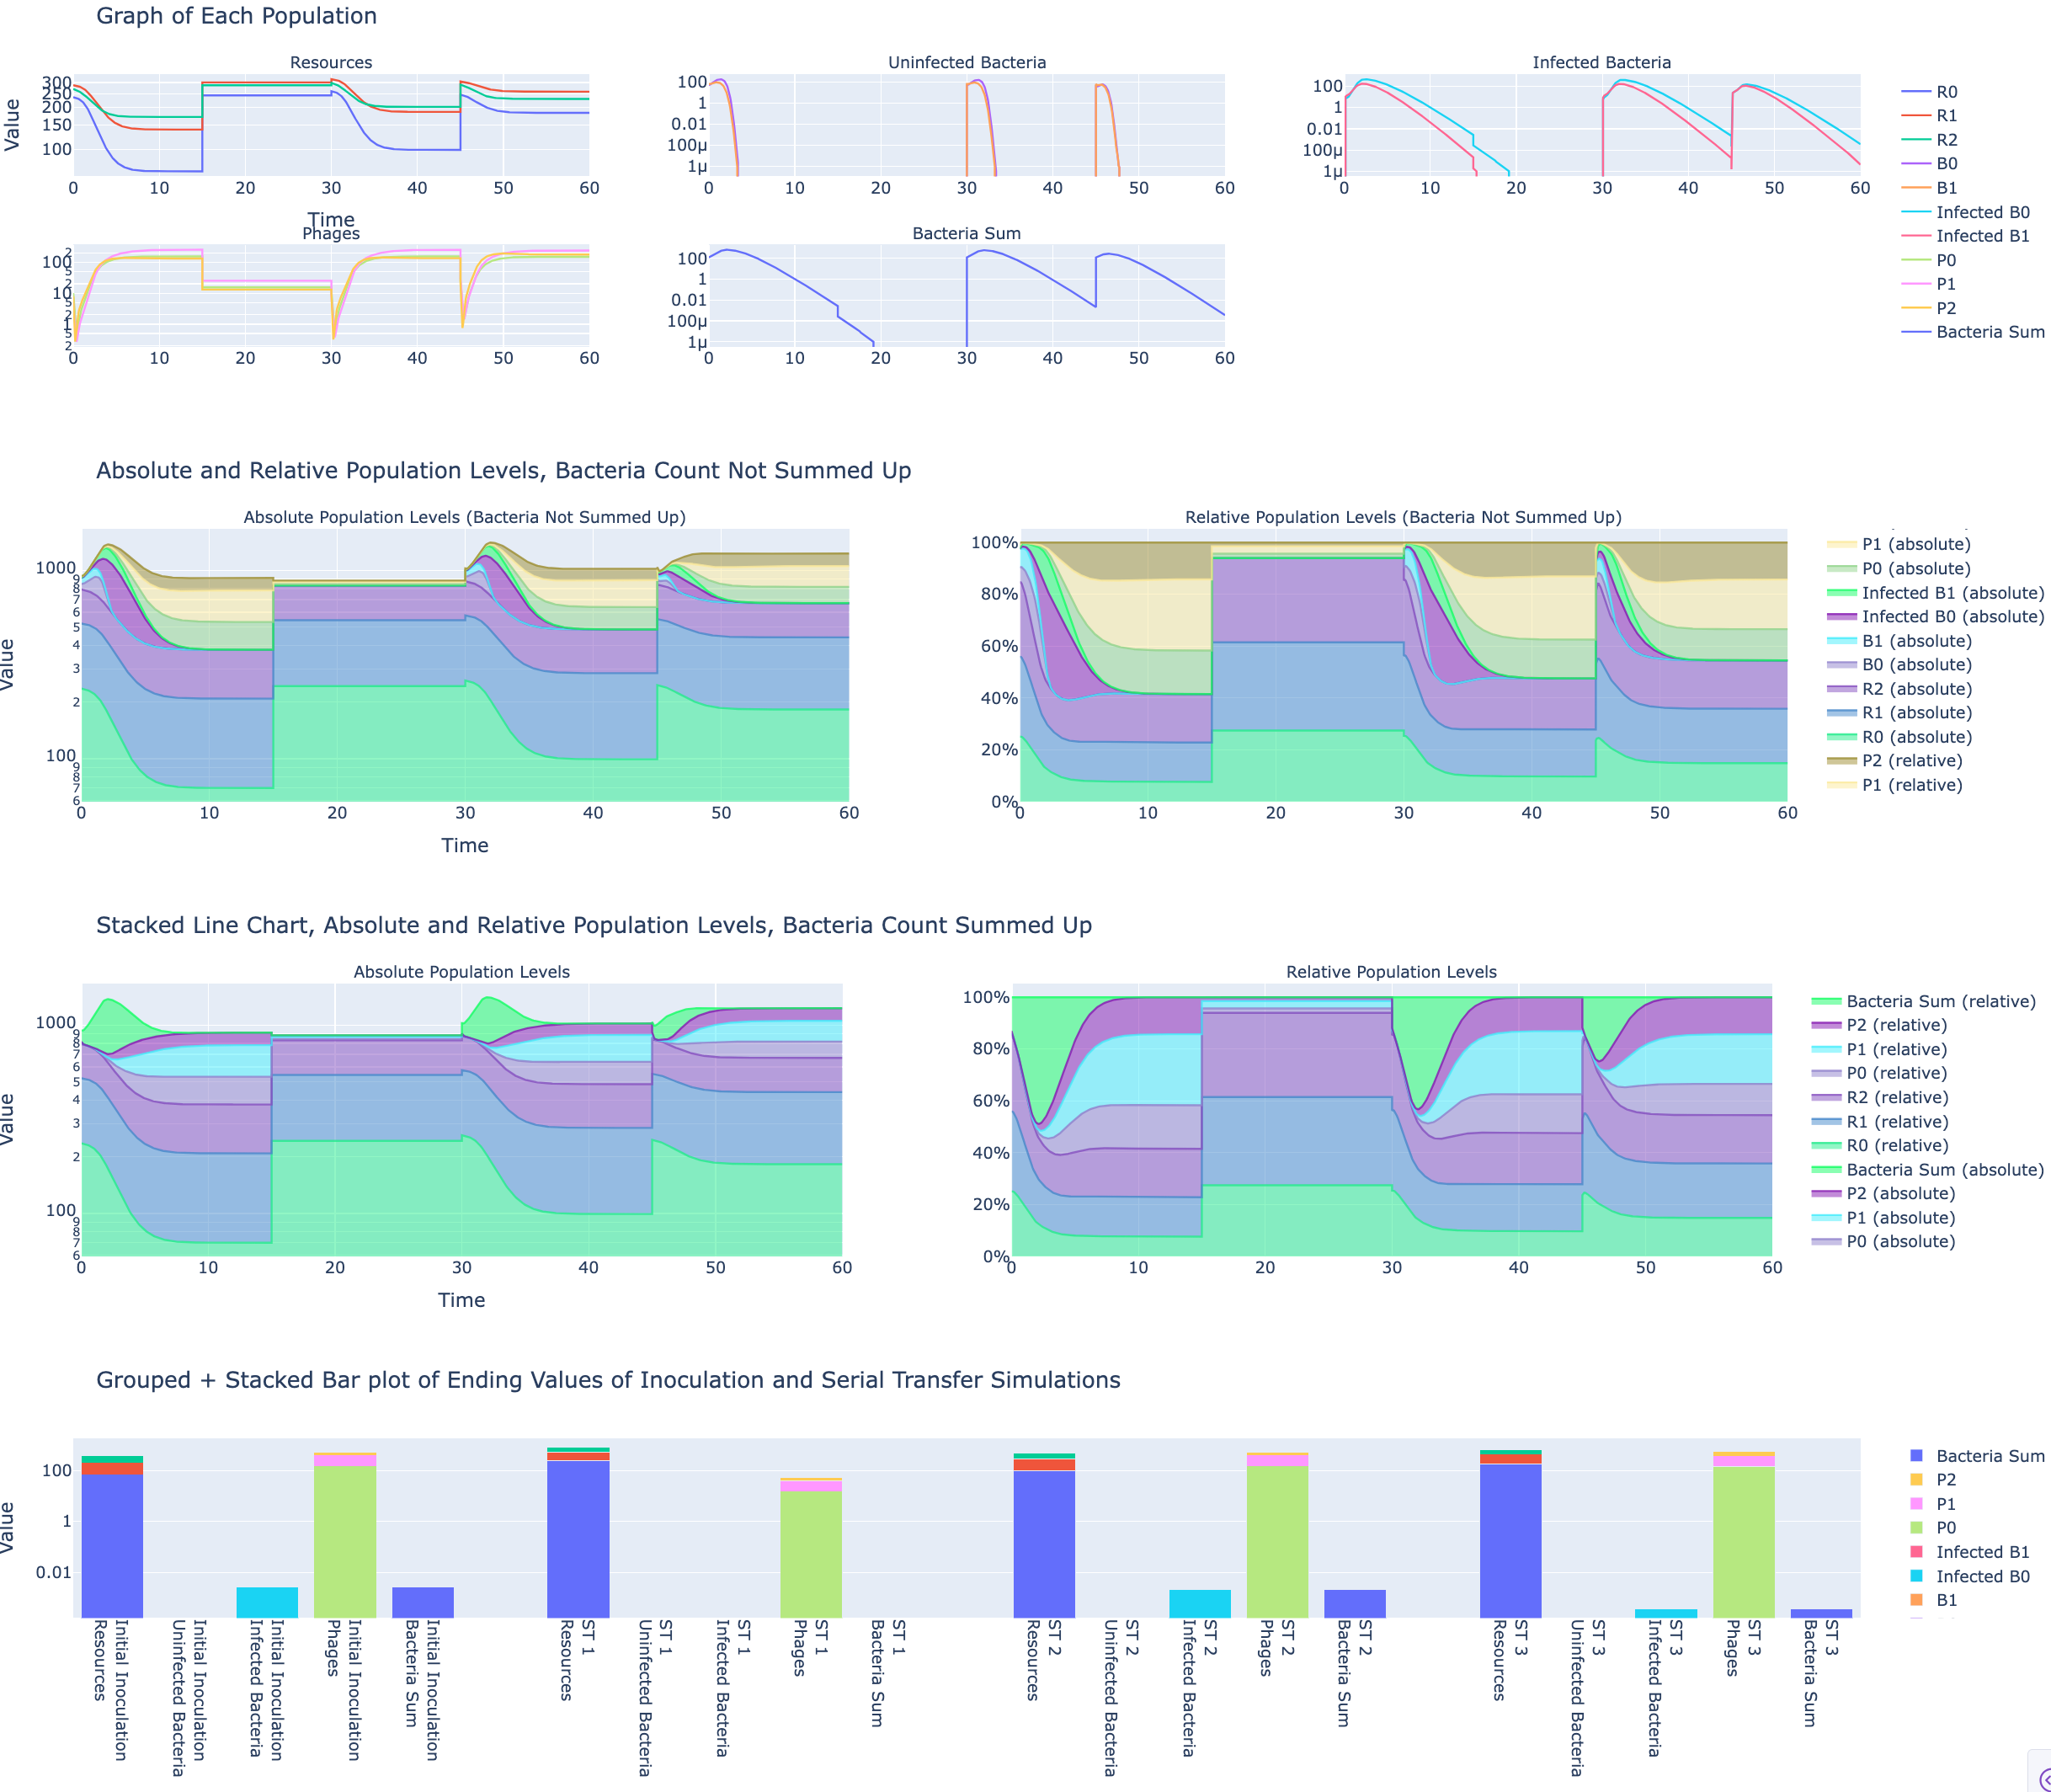
\includegraphics[width=\linewidth]{Screenshots/AdvancedVisualization/serial_transfer_run.png}
        \caption{
            The output plots of serial transfer. 
        }
        \label{fig:ss:av:serial_transfer_run}
    \end{subfigure}
    \caption{Serial Transfer}
 \end{figure}

\paragraph{Parameter Analysis}
\label{sec:parameter_analysis}
The parameter analysis settings tab as shown in \Cref{fig:ss:av:parameter_analysis_settings} allows the user to choose two parameters and individually run the model with the varying input values.
The values that can be tested and changed include all initial condition values, vector and matrix data, and environmental data.
As input, the user can select 2 parameters of choice.
After the parameter name selection, the user can manually choose which parameter values they want to test or test a range of values equally spaced by selecting the number of values to test.
Finally, the user can optionally run a serial transfer, where the serial transfer uses the settings found on the Serial Transfer tab. 

\Cref{fig:ss:av:parameter_analysis_run} shows the heatmap that the user can expect, one heatmap for each agent type.
Each heatmap cell represents the input of 2 unique parameter values, and shows the population count for that parameter run at the time shown in the slider. 
As the user slides the slider, the value inside the cell updates to correspond with the selected time. 
Note that the heatmap color range resets for each heatmap, so similar colors across heatmaps and across time will not correspond to the same values.

\begin{figure}[!ht]
    \centering
    \begin{subfigure}{0.49\linewidth}
        \centering
        \captionsetup{width=1\linewidth}
        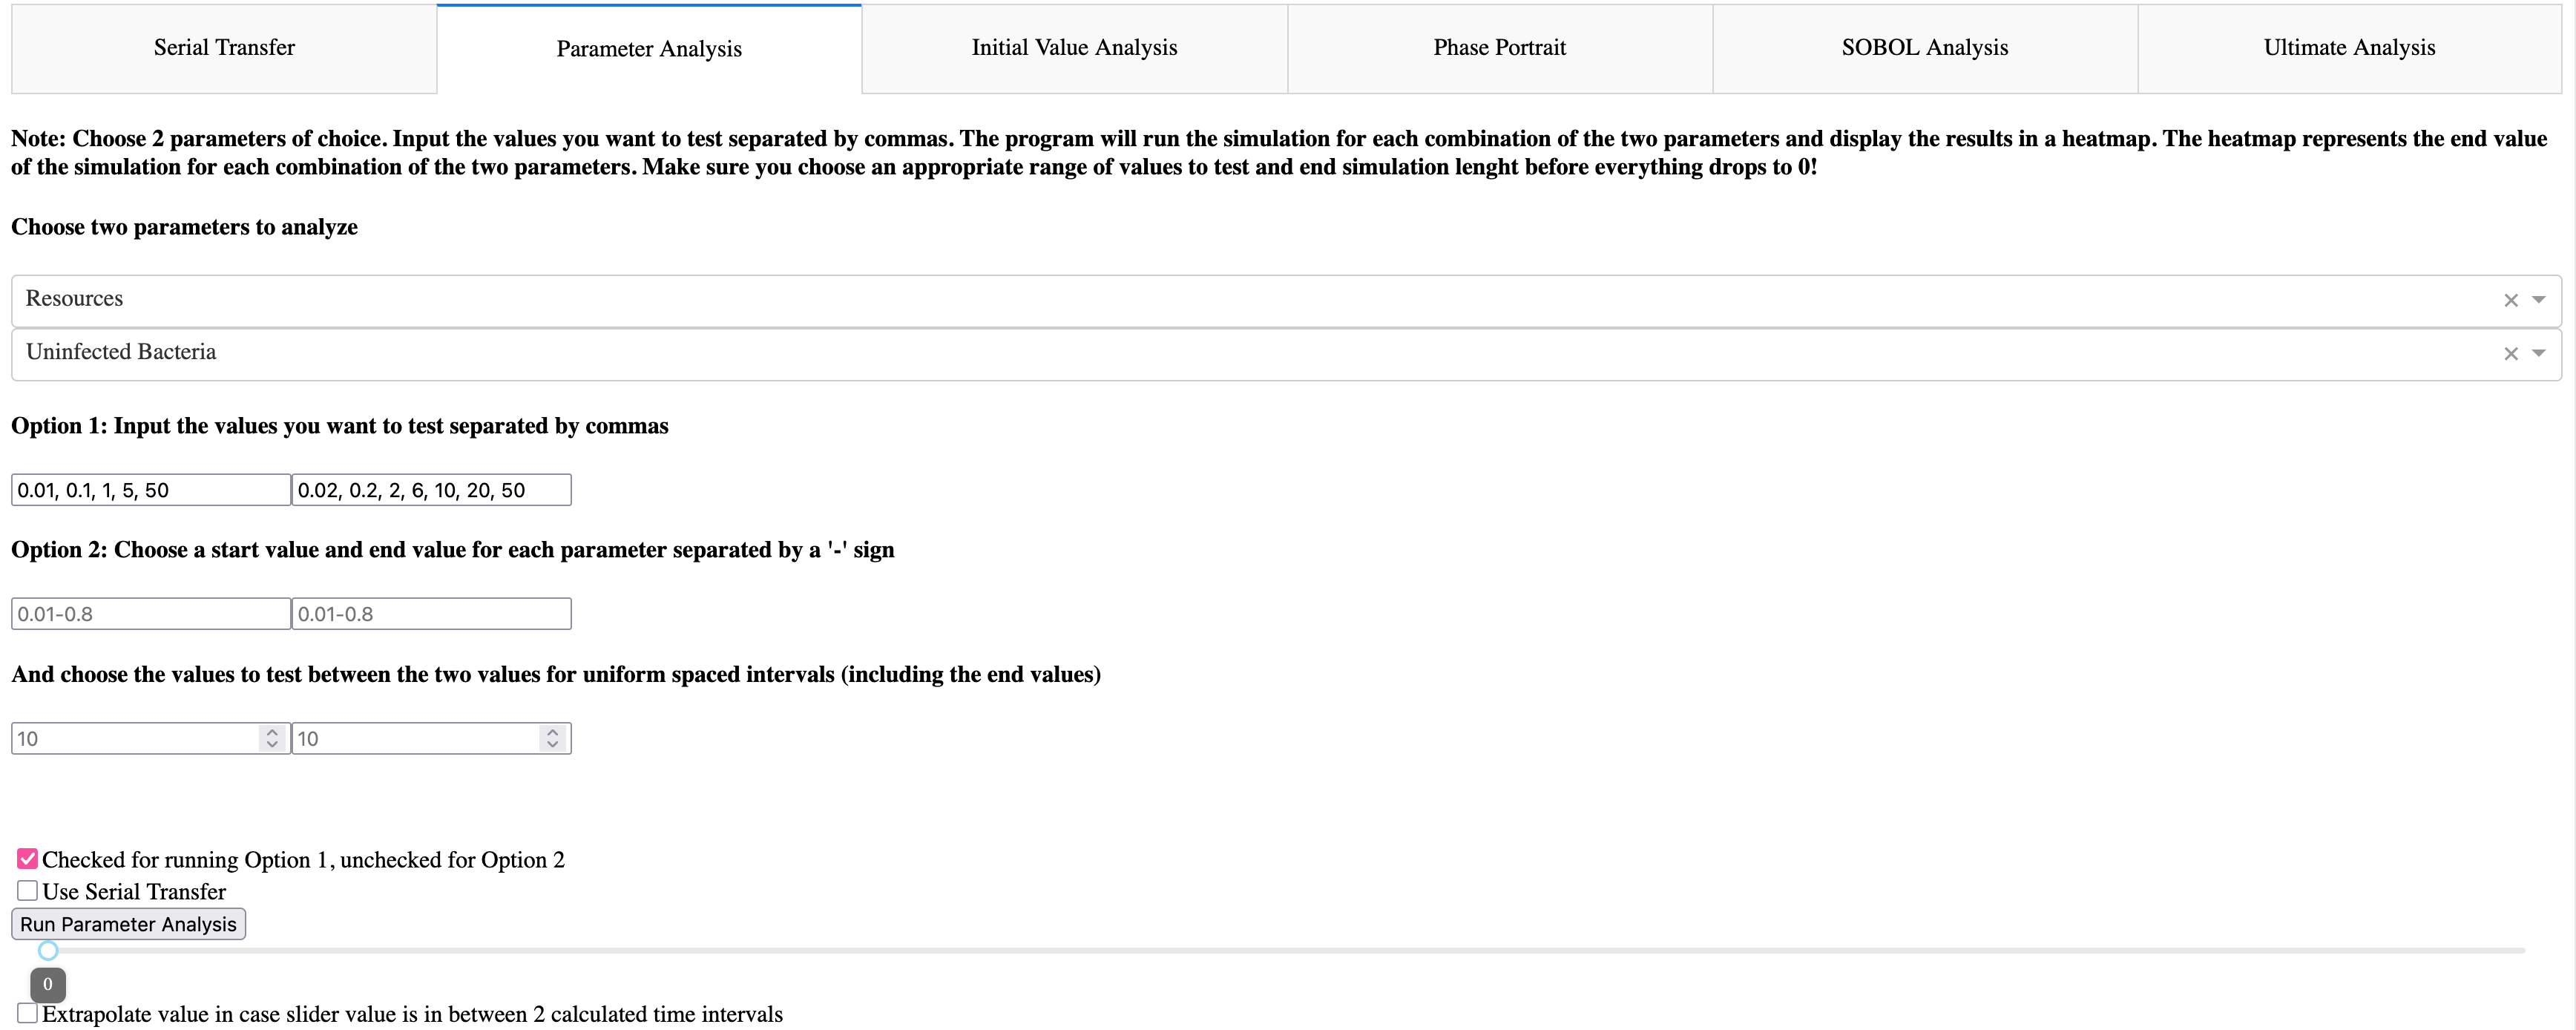
\includegraphics[width=\linewidth]{Screenshots/AdvancedVisualization/parameter_analysis_settings.png}
        \caption{
            The options available for the parameter analysis. 
        }
        \label{fig:ss:av:parameter_analysis_settings}
    \end{subfigure}
    \hfill
    \begin{subfigure}{0.49\linewidth}
        \centering
        \captionsetup{width=1\linewidth}
        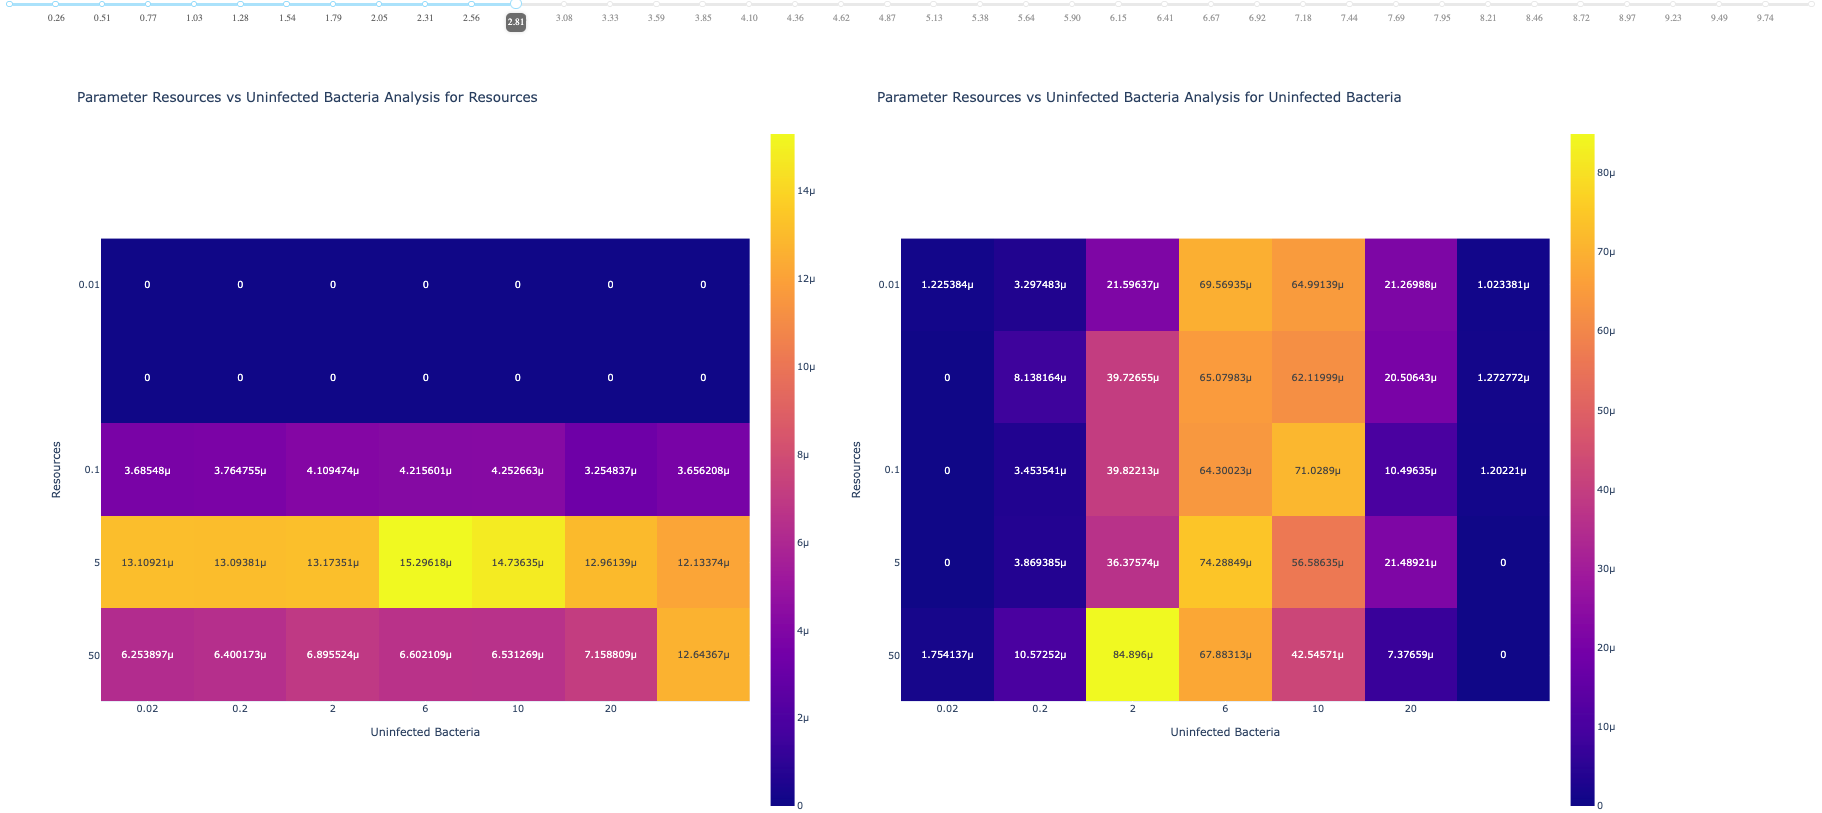
\includegraphics[width=\linewidth]{Screenshots/AdvancedVisualization/parameter_analysis_run.png}
        \caption{
            The output that the user can expect
        }
        \label{fig:ss:av:parameter_analysis_run}
    \end{subfigure}
    \caption{Parameter Analysis}
\end{figure}


\paragraph{Initial Value Analysis}
\label{sec:initial_value_analysis}
The initial value analysis settings tab as shown in \Cref{fig:ss:av:initial_value_analysis_settings} allows the user to choose a single parameter and vary the value of that parameter, visualizing how a change in parameter value affects the population count of the agents.

\Cref{fig:ss:av:initial_value_analysis_run} shows the plots that the user receives.
For each agent type, there are three plots made.
The left plot shows the population count through time, one line for each parameter value submitted.
The middle plot takes each run and calculates the “percentage from the max value“ (default value of $0.95 \rightarrow 95\%$) reached of the peak.
This value is considered the time of peak, and is used to fix some issues that can arise where the population plateaus or only keeps on rising.
The initial value is plotted on the x-axis, with the time at which the max value is reached on the y-axis.
Using the plotted data, a linear or log fit can be created.

The $R^2$ value, or coefficient of determination, is calculated as $R^2 = 1 - \frac{\sum_{i=1}^n (y_i - \hat{y}_i)^2}{\sum_{i=1}^n (y_i - \bar{y})^2}$
where $y_i$ is the observed values, $\hat{y}_i$ is the predicted values, and $\bar{y}$ is the mean of the observed values.

Using this data can be useful for understanding how a change in parameter value affects the time at which the population count reaches a maximum.
The slope, intercept and $R^2$ value is stored and saved in the third plot, a bar chart, with an editable name.
For every re-run of the initial value analysis, the slope, intercept and $R^2$ value is stored in the bar chart, allowing comparison of the slope-intercept data across different parameters. 

\begin{figure}[!ht]
    \centering
    \begin{subfigure}{0.49\linewidth}
        \centering
        \captionsetup{width=1\linewidth}
        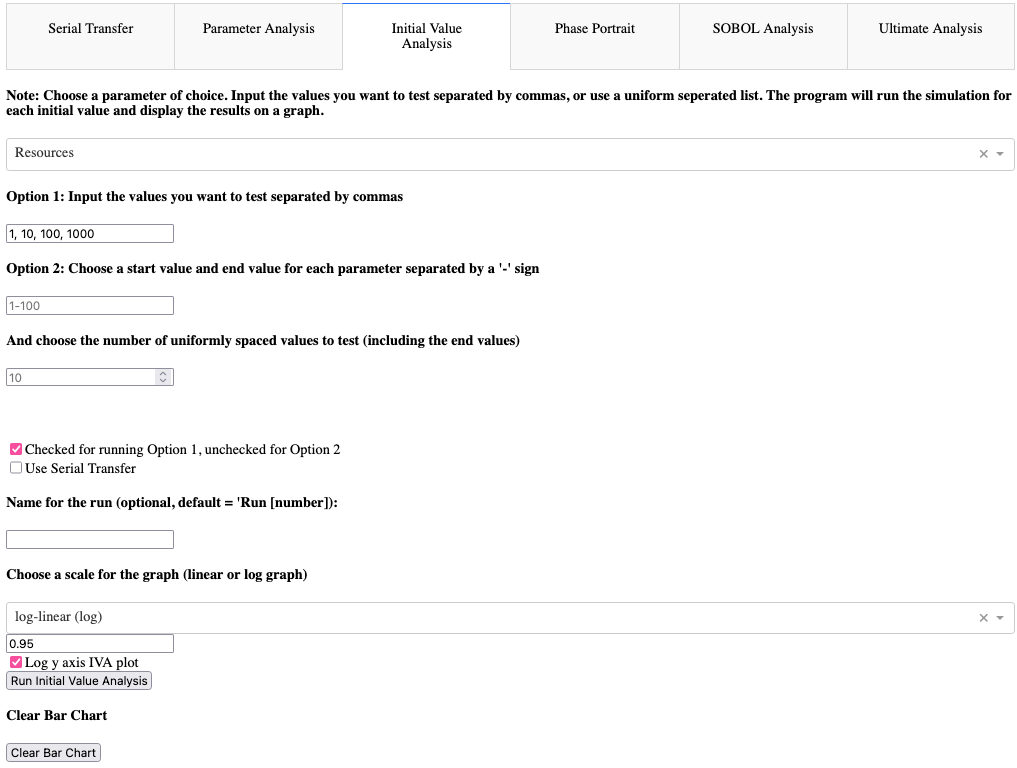
\includegraphics[width=\linewidth]{Screenshots/AdvancedVisualization/initial_value_analysis_settings.png}
        \caption{
            The settings for the initial value analysis tab. 
        }
        \label{fig:ss:av:initial_value_analysis_settings}
        \vspace*{\fill}
    \end{subfigure}
    \hfill
    \begin{subfigure}{0.49\linewidth}
        \centering
        \captionsetup{width=1\linewidth}
        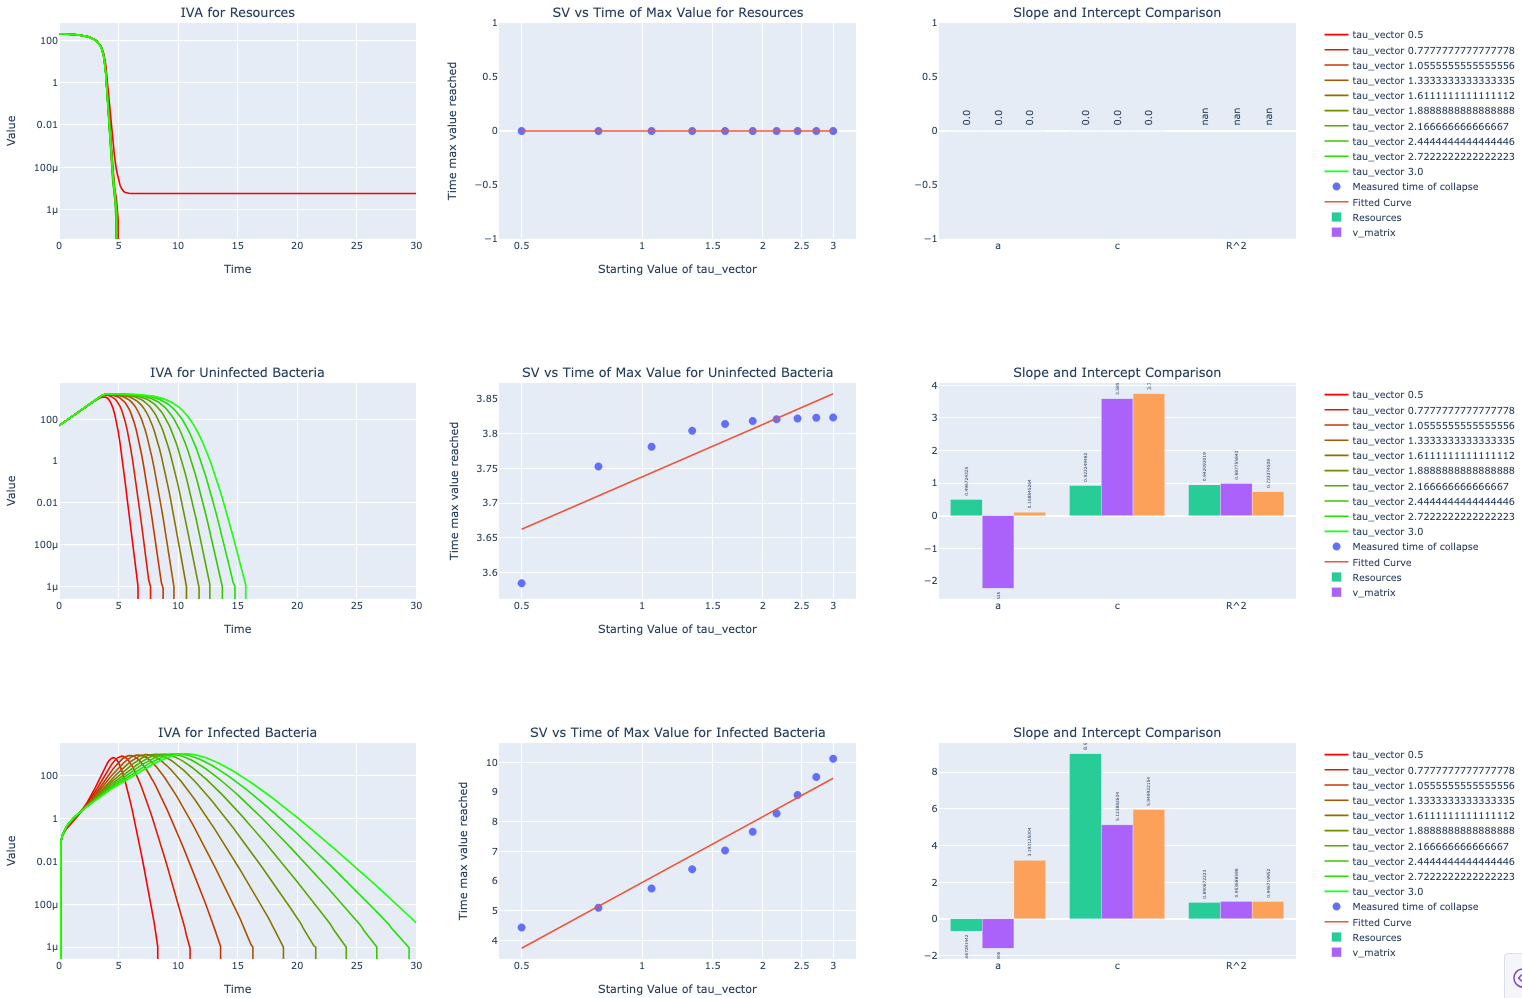
\includegraphics[width=\linewidth]{Screenshots/AdvancedVisualization/initial_value_analysis_run.png}
        \caption{
            An example initial value analysis output. 
        }
        \label{fig:ss:av:initial_value_analysis_run}
        \vspace*{\fill}
    \end{subfigure}
    \caption{Initial value analysis}
\end{figure}

\paragraph{Phase Portrait}
\label{sec:phase_portrait}
The phase portrait plot allows for the user to analyze how an agent population evolves with respect to the other agent population through time.
Phase portraits indicate how one population increases while the other decreases, and vice versa.
Steady states can be identified and classified as either stable, unstable, or as saddle points.
By comparing different starting points, it is possible to see if the system is chaotic or not.
The setup for the phase portrait can be seen in \Cref{fig:ss:av:phase_portrait_settings}, and a sample output can be seen in \Cref{fig:ss:av:phase_portrait_run}. 

\begin{figure}[!ht]
    \centering
    \begin{subfigure}{0.49\linewidth}
        \centering
        \captionsetup{width=1\linewidth}
        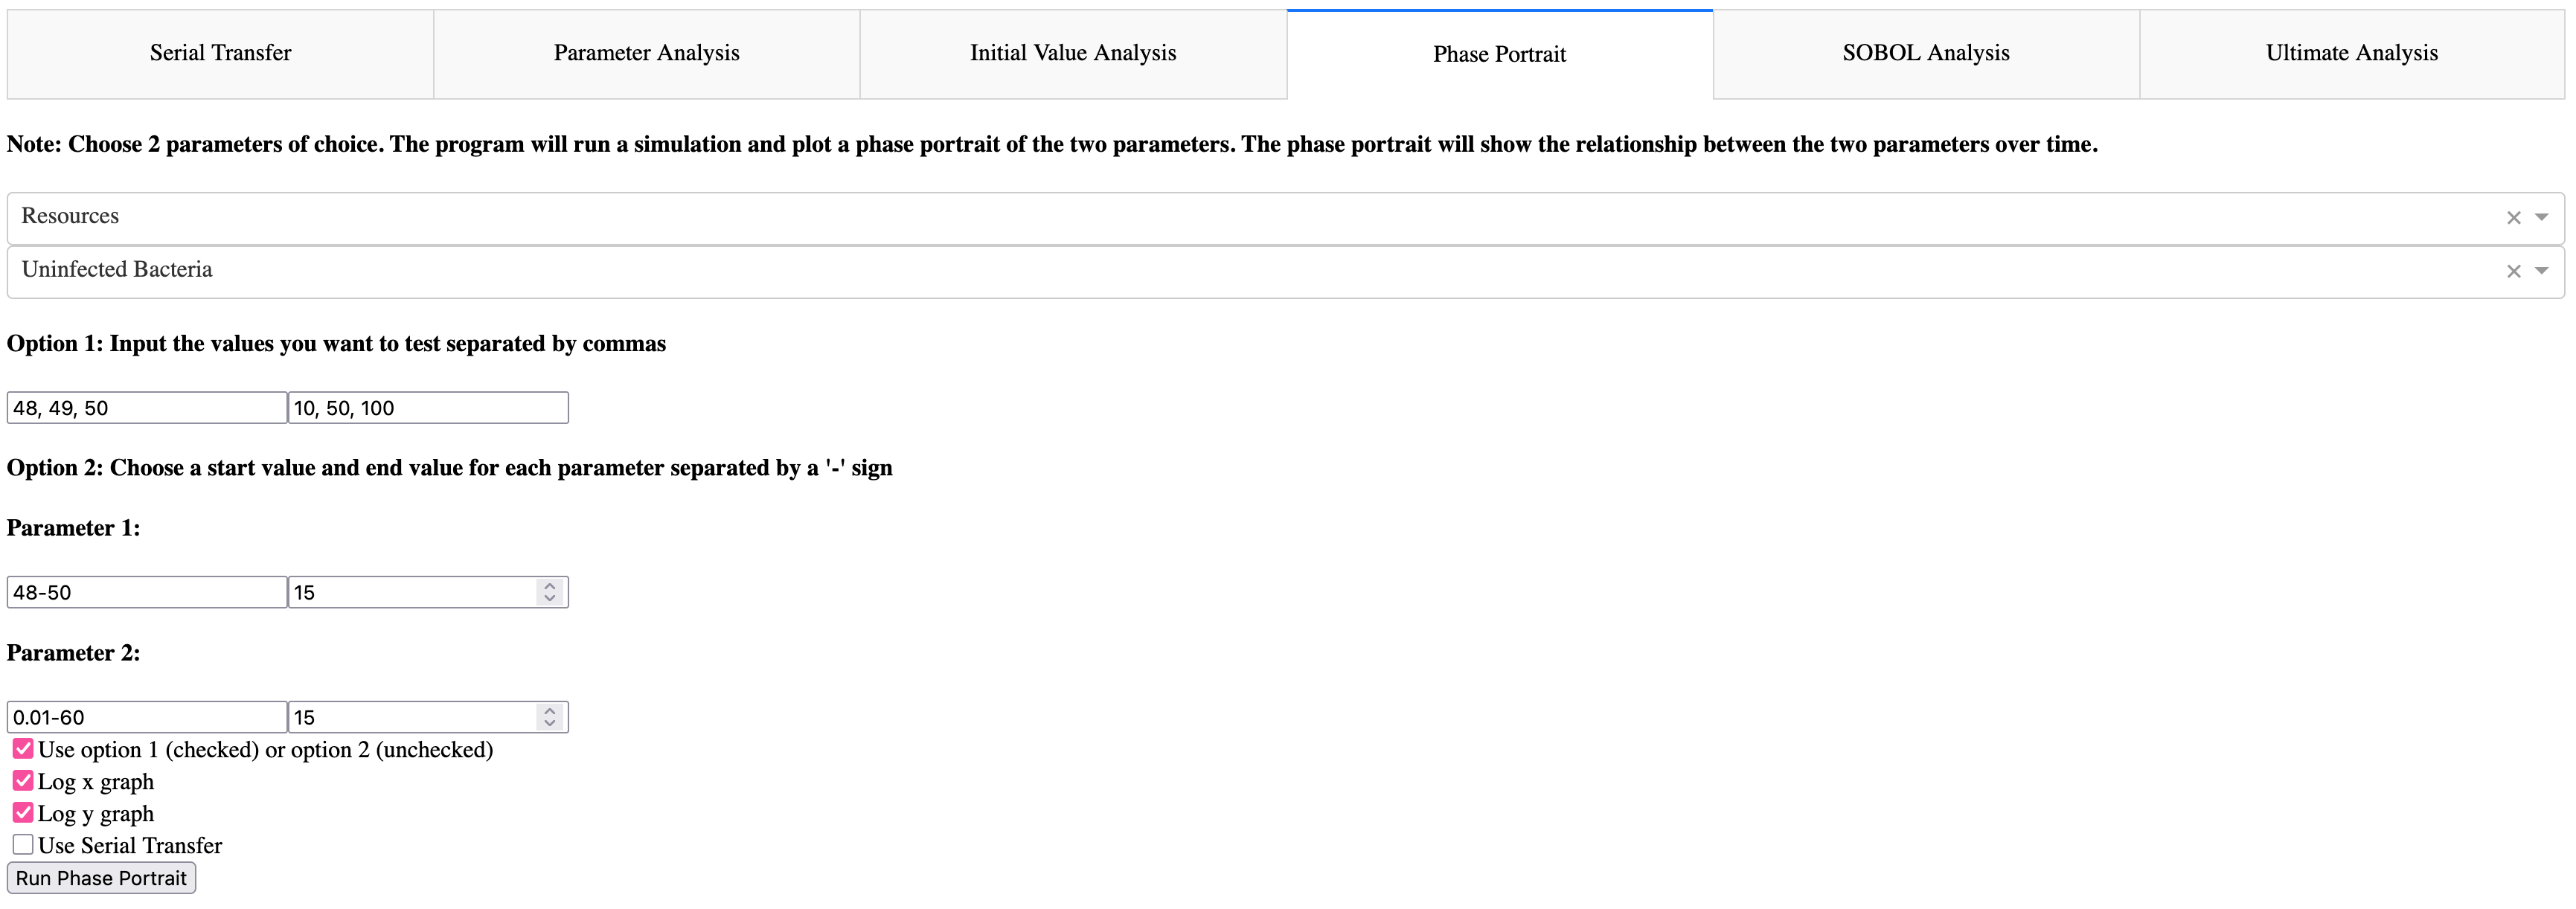
\includegraphics[width=\linewidth]{Screenshots/AdvancedVisualization/phase_portrait_settings.png}
        \caption{
            The user can select two starting values for the initial condition, but they can't choose vector, matrix, or environment settings due to the plot showing the development of agent populations against other agent populations.
            As typical, the user can select their own values or auto-generate values between two values, as well as use a serial transfer option.
            There is also an option to take the logarithm of the x and/or y-axis. 
        }
        \label{fig:ss:av:phase_portrait_settings}
    \end{subfigure}
    \hfill
    \begin{subfigure}{0.49\linewidth}
        \centering
        \captionsetup{width=1\linewidth}
        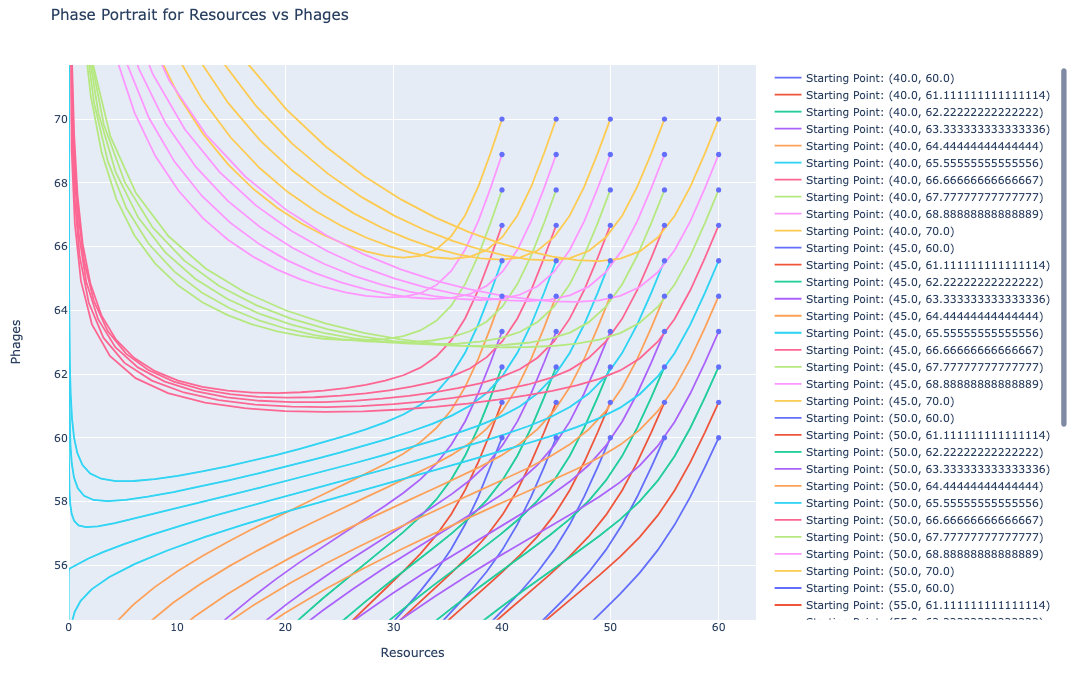
\includegraphics[width=\linewidth]{Screenshots/AdvancedVisualization/phase_portrait_run.png}
        \caption{
            An example run of a phase portrait.
        }
        \label{fig:ss:av:phase_portrait_run}
    \end{subfigure}
    \caption{Phase Portrait}
\end{figure}

\paragraph{SOBOL Sensitivity Analysis}
\label{sec:SOBOL_sensitivity_analysis}
SOBOL analysis, a variance-based sensitivity analysis, is a method that allows a user to quantify how important an input parameter has on a measured aspect of the output by changing the parameter values of the model and measuring the change in model output.
SOBOL quantifies how much variance in the output can be attributed to a specific parameter and can measure the effect of global/total ($ST$), first ($S1$), and second order sensitivity ($S2$). 
Global, also called total sensitivity, is the summation of all higher order interactions. 
First order $Si$, or local sensitivity, is the measurement of the effect that parameter $i$ has on the variance of the output. 
Second order is the measurement of parameter $i$ interacting with parameter $j$, nad how the interaction attributes to the output variance. 
Etc for third order and higher. 
When $ST_i >> S1_i$ then parameter $i$ depends on interactions with other parameters, while when $ST_i \equiv S1_i$, then $i$ doesn't interact much with and depend on other parameters.
It should be stated that $ST_i \geq S1_i$. 

When a model is viewed as a black-box model, the model can be seen as a function $Y=f(X)$, where $X$ is an input vector of $d$ elements, and $Y$ is a univariate model output.
$X$ is assumed to be independently and uniformly distributed within a hypercube $X_i \in [0, 1]$ for $i=1, \dots d$.
The first order sensitivity measures the output variance of the main affect of parameter $X_i$.
Measuring the effect of varying $X_i$ averaged over other input parameters, and standardized to provide a fractional contribution to the overall output variance.
The first order sensitivity is described as
\[
    S1_i = \frac{V_i}{\textit{Var}(Y)}
\] where $V_i = \textit{Var}_{X_i}(\mathbb{E}_{X_{\sim i}}[Y|X_i])$ and where $X_{\sim i}$ represents all the parameters that are not $X_i$.
All parameters are summarized in \Cref{tab:parameter_table_SOBOL}

The second order index measures the impact of input $X_i$ interacting with $X_j$. For many inputs, this becomes unwieldy to analyze.
The global sensitivity is used to analyze the global sensitivity without evaluating $2^d-1$ indices, and measures the contribution to the output variance of $X_i$, including all variance due to $X_i$'s interaction with other variables.
\[
    S1_i = \frac{\mathbb{E}_{X_{\sim i}}[\textit{Var}_{X_i}(Y|X_{\sim i}))}{\textit{Var}(Y)} = 1 - \frac{\textit{Var}_{X_i}(\mathbb{E}_{X_i}[Y|X_{\sim i}])}{\textit{Var}(Y)}
\]
SOBOL can analyze various univariate outputs.
This could be either the average value of an agent population, the variance in population count, the time at the peak of an agent count, the final population value, etc. \newline
SOBOL accepts a list of parameter names and a list of range of values to sample from, which the user can input in the SOBOL settings tab, \Cref{fig:ss:av:SOBOL_analysis_settings}. 
If no values are added, the parameter is not included in the simulation and the default value is instead used. 
The user then needs to select the number of samples to run, using the formula $2^x$, where $x$ is the number they input, and $2^x$ is the number of samples that SOBOL will create and run.
The larger $x$ is, the more accurate the SOBOL analysis results will be, but the more simulations would need to be run. \newline
Otherwise, if 2nd order is not chosen, the model is run $N(D+2)$ times.
If the user wants to analyze the second order interactions, then the model will run the system $N(2D+2)$ times with the randomly sampled input values, where $N$ is a multiple of 2, and $D$ is the number of parameters being tested.
Due to the randomness of the sampling method, the user can, but does not need to, submit a seed value. 

Three SOBOL analyses are included by default in the dashboard, as shown in \Cref{fig:ss:av:SOBOL_analysis_run}.
An analysis of the final value of the simulation, the average population count, and the variance in population count.
The global and first sensitivity are shown next to one another, and each sub-row within a plot represents each agent type. 
The proportion of the global and local sensitivity can be seen for each agent type and each parameter.

It can be argued that the final, average, and variance value of the run is not a useful statistic to measure and run a SOBOL analysis on. 
One might give the reasoning that the population value at time $t$ depends on the previous time step $t-1$. 
Thus the average and variance of the value is not completely random and is semi dependent on the previous value. 
Another argument is that the simple golden model doesn't exhibit complex behavior unlike the output exhibited in \Cref{fig:cocktail_plot}. 

Making a dashboard that can be used for different inputs is hard to make. Predicting the type of plots that a user might be interested in, and the type of behavior the user wants to analyze is impossible to predict. 
Therefore, three simple and easy to understand default SOBOL analysis methods are provided that aims to capture the simple dynamics of the system. 
Upon completion of a SOBOL analysis, the original simulation data is stored to the disk as a \textit{.pickle} file so that the user can use the data and run their own SOBOL analyses. 

\begin{figure}[!ht]
    \centering
    \begin{subfigure}{0.49\linewidth}
        \centering
        \captionsetup{width=1\linewidth}
        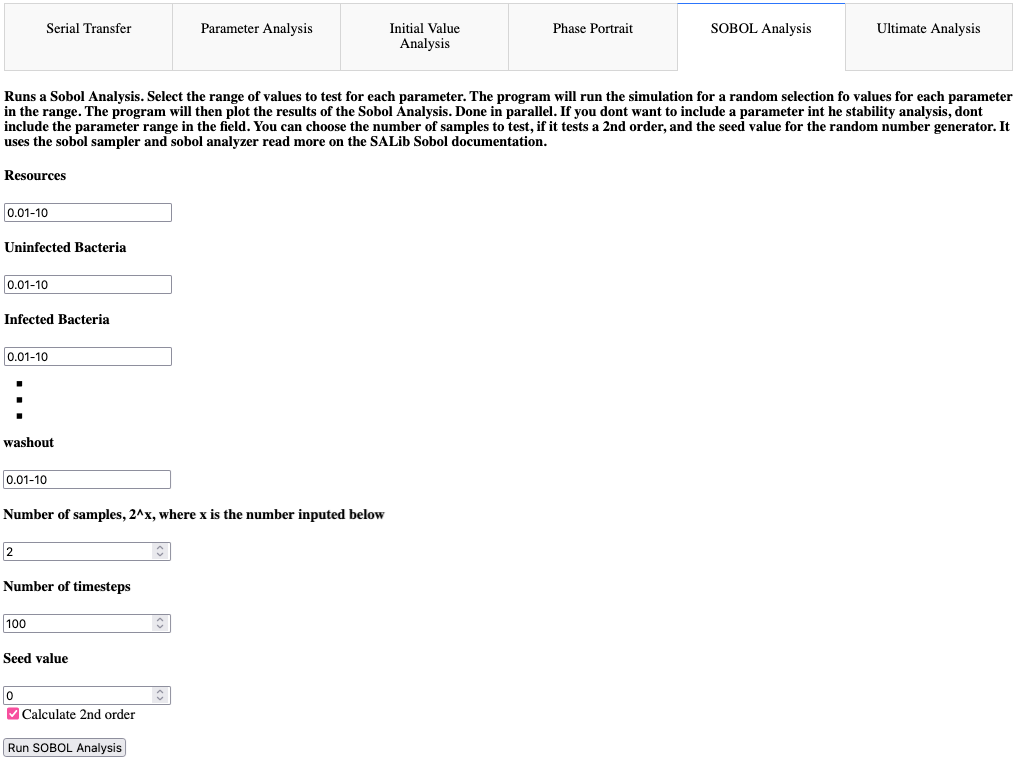
\includegraphics[width=\linewidth]{Screenshots/AdvancedVisualization/SOBOL_analysis_settings.png}
        \caption{
            The SOBOL settings tab. 
        }
        \label{fig:ss:av:SOBOL_analysis_settings}
    \end{subfigure}
    \hfill
    \begin{subfigure}{0.49\linewidth}
        \centering
        \captionsetup{width=1\linewidth}
        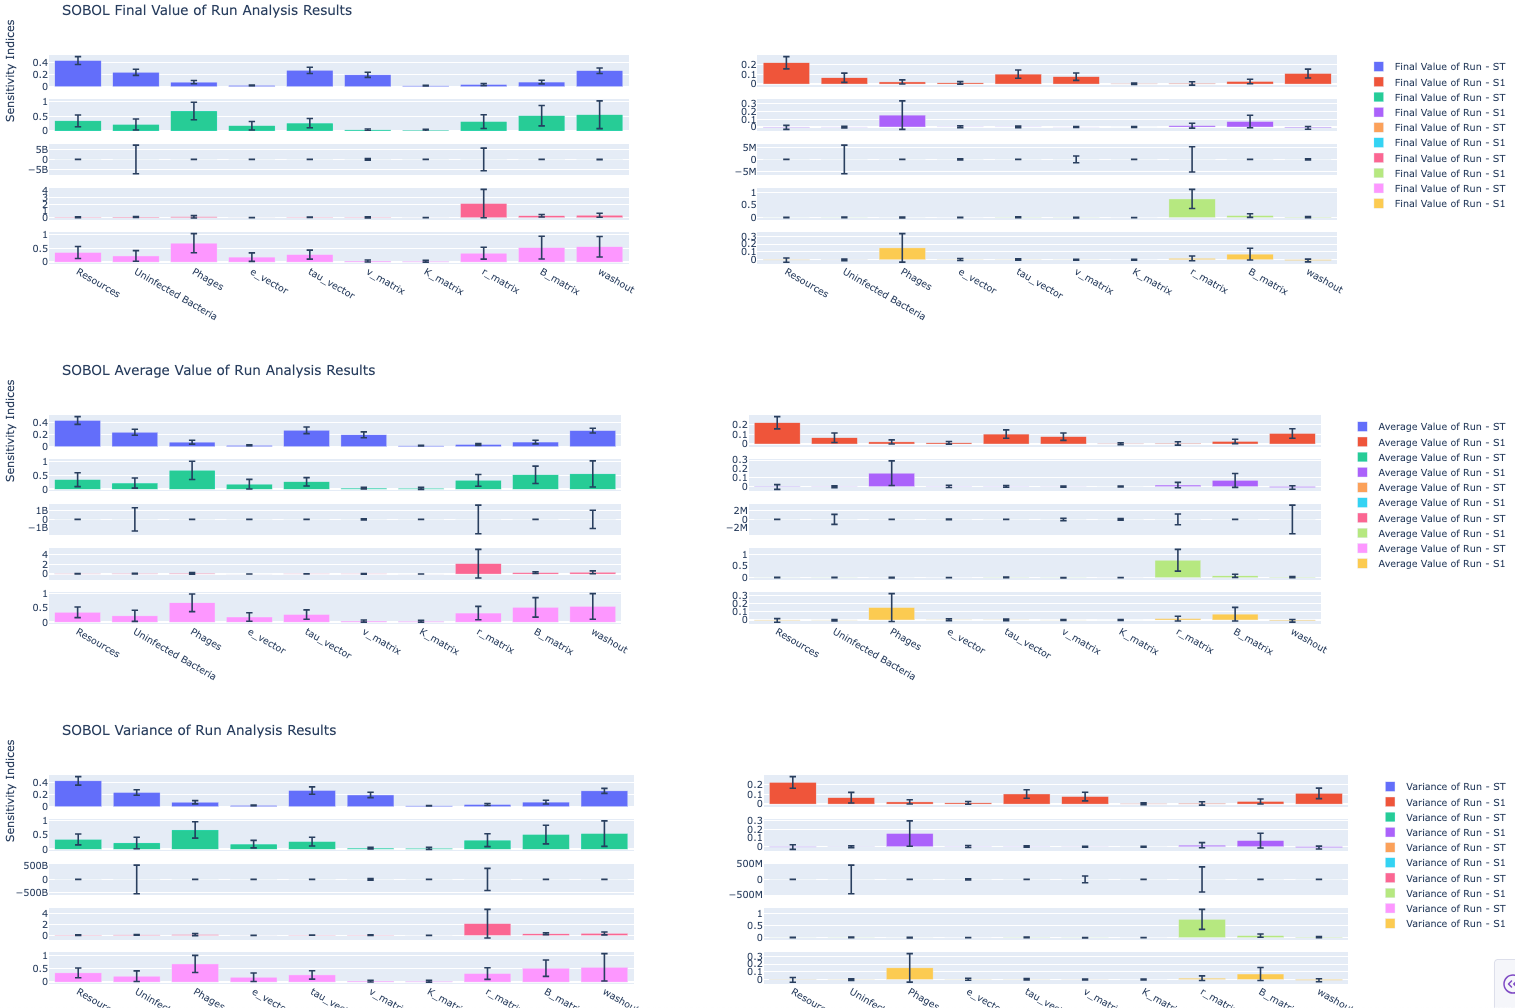
\includegraphics[width=\linewidth]{Screenshots/AdvancedVisualization/SOBOL_analysis_run.png}
        \caption{
            The output that can be expected from SOBOL. 
        }
        \label{fig:ss:av:SOBOL_analysis_run}
    \end{subfigure}
    \caption{SOBOL variance analysis}
\end{figure}

\paragraph{Ultimate Analysis}
\label{sec:ultimate_analysis}
The Ultimate Analysis section does not produce any visualizations or analysis, but instead allows for the user to define which initial conditions and parameter values they want to run a simulation on.
The solver will iterate over every single parameter input possibility and save the results in a \textit{.parquet} file.
Similarly settings in the other sections, the user can specify a start and end value, along with the number of values to generate evenly spaced within that range, including both the start and end values (\Cref{fig:ss:av:ultimate_analysis_settings}).
\newline
Using Dask and the saved \textit{.parquet} file, the user can query for specific runs, for example runs where a parameter value was greater than 0.05, and use the simulation data to create their own plots.
\begin{figure}
    \centering
    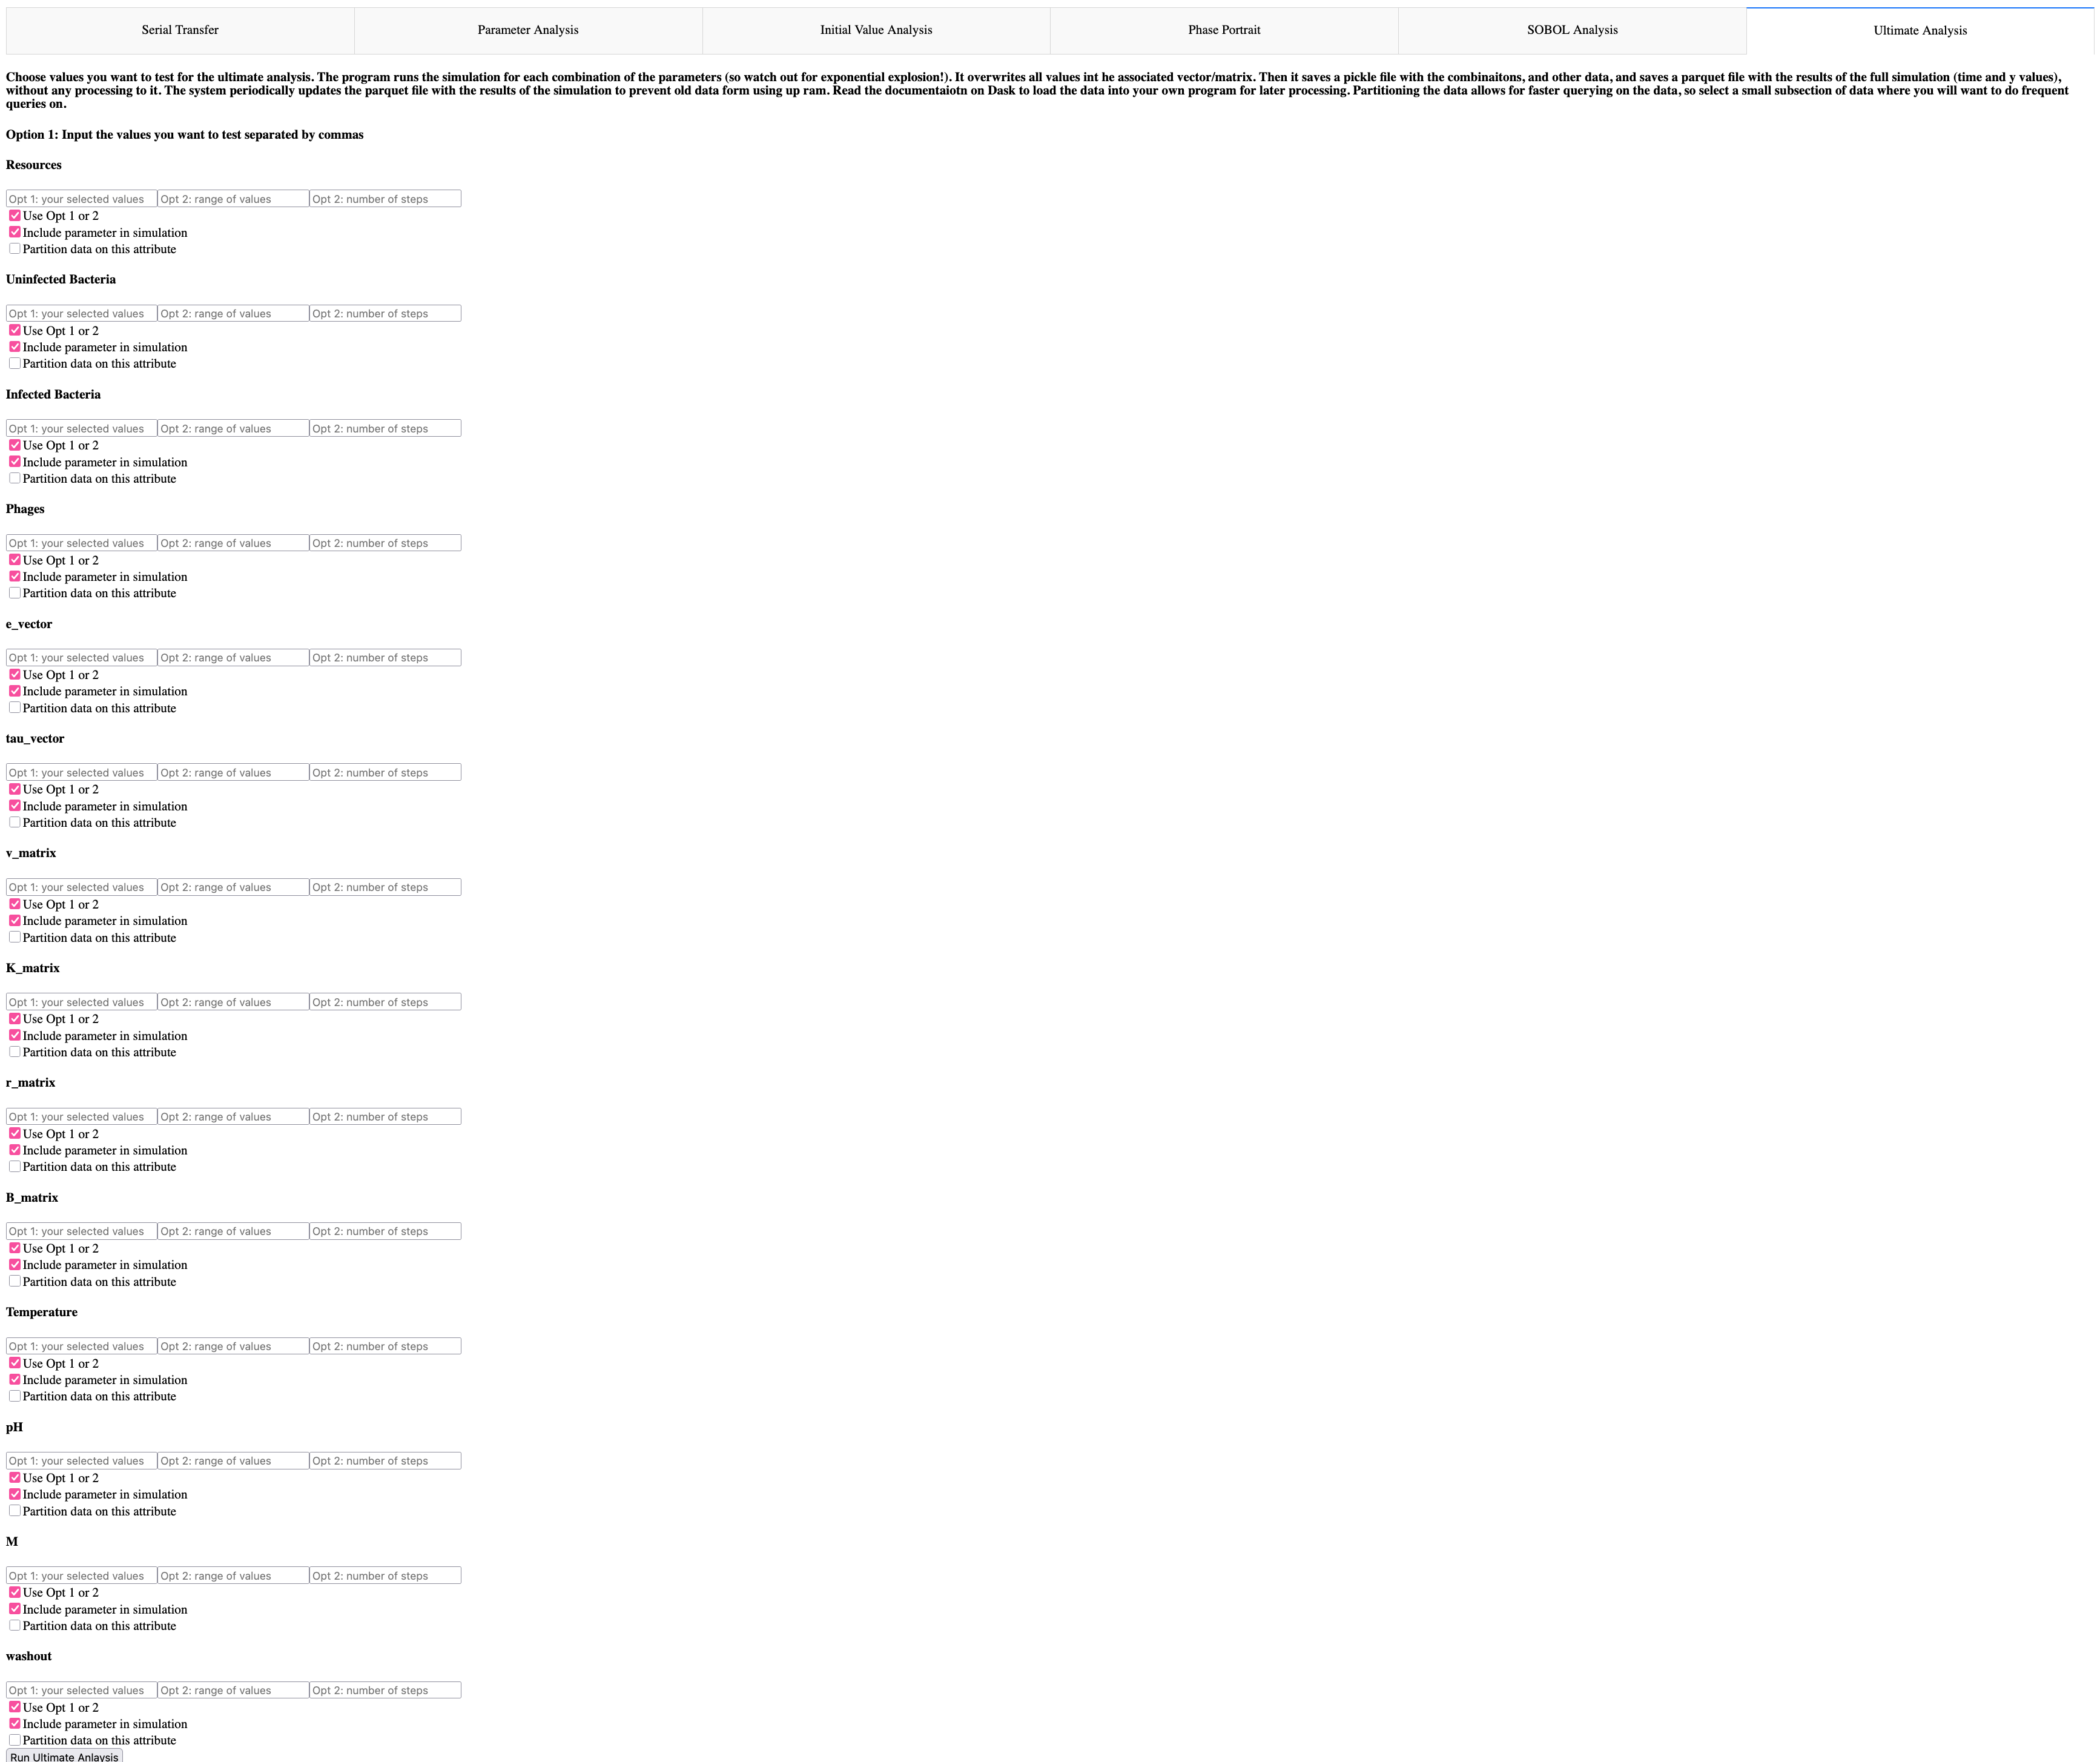
\includegraphics[width=1\linewidth]{Screenshots/AdvancedVisualization/ultimate_analysis_settings.png}
    \caption{
        The ultimate analysis setup tab. 
    }
    \label{fig:ss:av:ultimate_analysis_settings}
\end{figure}

\subsection{Custom Visualizations and Analyses} 
\label{sec:custom_visualizations_and_framework}
The final part, an optional step, allows the user to define a number of parameters they want to simulate and download the simulation results. 
The user can use this data to create their own custom visualizations without having to rerun the simulations, especially if there are many simulations. 
The data can be further processed and visualized as the user wishes. 

Depending on the provided model, different behavior might appear. 
As the dashboard can not create a graph for every situation, or be easily adapted to analyze every situation, \nameref{sec:ultimate_analysis} can be used to run and download the simulation data to the disk to later create your own custom visualizations. 
For example the agents in a model can exhibit cyclic behavior. 
A custom visualization that the could be created for this cyclic model would be to perform a Fourier transformation on the curve to obtain the predominant frequencies. 
A change in parameter values would change the frequencies of the curve, so it would be easy to quantify how a change in parameter value affects the frequency output. 
If dampening occurs, then a change in amplitude can also be measured, and compared to the change in frequency, allowing the user to identify if the frequency-dampening relationship is correlated or not. 

\section{Software Used and Packages}
The program was created exclusively in Python \cite{Python}, and makes extensive usages of various packages, ranging from the standard scientific packages such as NumPy \cite{NumPy} and SciPy to more niche packages such as pickle and SALib \cite{iwanagaSALib20Advancing2022, hermanSALibOpensourcePython2017}.

The graphical tool uses Tkinter acting as the front end, handling the user inputs, while NetworkX \cite{hagbergExploringNetworkStructure2008} stores the graph and contains the attribute data. 
The GUI tool also uses Matplotlib \cite{Matplotlib}to create the figure of the graph to display to the user in the GUI tool.

The simulation framework, the backend of the modelling, makes extensive usage of SciPy's \textit{solve\_ivp()} to create the ODE data. 
It also makes light usage of NetworkX to load the graph, as it initially takes a graph as an input, and light usage of NumPy to setup the parameters at startup. 

The visualization part makes heavily usage of Dash and Plotly. 
Dash acts as the server and is used for displaying the HTML aspect of the frontend and dealing with any input and output. 
Upon choosing parameter values and clicking on “submit“, Dash registers the activity and calls the function registered to the button, sending data such as parameter values and options like "log x-axis" form the frontend to the backend server. 
In the backend, the various inputs are handled, like changing the input string “0.05, 0.1, 0.15, 0.2” into an iterable list [0.05, 0.1, 0.15, 0.2] that the simulation framework can iterate over to vary the parameter value. 

If there are many simulations to run through, in the case of \nameref{sec:ultimate_analysis}, an intermediate call to a parallel computing library Joblib is called, where Joblib parallelizes the for-loop to compute the simulations in parallel. 

Ultimate analysis uses Pandas to write the data to a \textit{.parquet} file. 
Pandas parquet offers efficient data compression, efficient memory usage and when combined with Dask, efficient querying functionalities in a Dataframe format that many data scientists would be familiar with. 

SOBOL uses the SALib library to sample and analyze the parameter input. 
Both ultimate analysis and SOBOL save a \textit{.pickle} file containing a dictionary with the parameter values tested, setting values, and other important information regarding the simulation. 

\nameref{sec:initial_value_analysis} uses SciPy's \textit{curve\_fit()} function to curve fit the points in the middle plot (\Cref{fig:ss:av:initial_value_analysis_run}). 

Other packages that are used include collections, copy, warnings, itertools, os, datetime, json, gc, and time. 
\newpage

\section{Experiments and Results}
    \label{sec:Experiments}
    freds
    \newpage

\section{Discussion}
    \label{sec:Discussion}
    \chapter{Discussion}
\label{Discussion}
    \newpage

\section{Conclusion and Future Work}
    \label{sec:Conclusion}
    frefre
    \newpage
rgtggrt
\printbibliography[heading=bibintoc, title={References}]
\newpage

\appendix 
\section{Parameters}
    \label{sec:Parameters}
    Parameters used in equations

\begin{table}[ht!]
    \begin{tabular}{|l|p{3.5cm}|p{4cm}|l|l|l|}
        \hline
        Parameter & Parameter Full Name & Description & Default Value & Alternatives & Notes \\ \hline
        ${P}$ & Phage Parameter & Phage population count & & & \\ \hline
        ${U}$ & Unifected Parameter & Uninfected bacteria population count & & & \\ \hline
        ${I}$ & Infected Parameter & Infected bacteria population count & & & \\ \hline
        ${R}$ & Resource Parameter & Resource concentration & & & \\ \hline
        ${B}$ & Bacteria Parameter & Bacteria population & & & Some models explicitly model uninfected and infected bacteria, ${B} = {U} + {I}$ \\ \hline
        $\omega$ & Washout Rate & Rate of parameter washing or flowing out of the system & & & \\ \hline
        $\beta$ & Burst Size & Number of phages created when bacteria cell bursts & & & \\ \hline
        $t$ & Time & Time step during simulation &  &  & \\ \hline
        $\mu$ & Mean & Mean &  &  & \\ \hline
        $\sigma$ & Standard Deviation & Standard deviation &  &  & \\ \hline
        $T_{min}$ & Minimum Temperature & Minimum operating temperature for a microbe &  &  & \\ \hline
        $T_{opt}$& Optimal Temperature & Optimal operating temperature for a microbe &  &  & \\ \hline
        $T_{max}$& Maximum Temeprature & Maximum operating temperature for a microbe &  &  & \\ \hline
        $pH_{min}$& Minimum pH & Minimum operating pH for a microbe &  &  & \\ \hline
        $pH_{opt}$& Optimal pH & Optimal operating pH for a microbe &  &  & \\ \hline
        $pH_{max}$& Maximum pH & Maximum operating pH for a microbe &  &  & \\ \hline
    \end{tabular}
\end{table}
    \newpage

\section{Appendix 1}
    \label{sec:Appendix1}
    Due to the nature of killing bacteria, there are numerous applications where a researcher or an organization might be interested in controlling bacterial populations.

A Food Safety Specialist might be interested in introducing a solution containing a high concentration of phages during food production to prevent the spread and growth of \textit{Salmonella} or \textit{E. coli} in the pet food.  
Alternatively, the Food Safety Specialist might want to promote beneficial bacteria like \textit{Streptococcus thermophilus} used in the production of Emmental cheese, which heat would kill when the milk undergoes the pasteurization process. 

Phages offer properties of microbial control that other methods do not, making them an ideal candidate for some applications. 
    \newpage
\end{document}